\documentclass[
  jou,
  floatsintext,
  longtable,
  nolmodern,
  notxfonts,
  notimes,
  colorlinks=true,linkcolor=blue,citecolor=blue,urlcolor=blue]{apa7}

\usepackage{amsmath}
\usepackage{amssymb}




\RequirePackage{longtable}
\RequirePackage{threeparttablex}

\makeatletter
\renewcommand{\paragraph}{\@startsection{paragraph}{4}{\parindent}%
	{0\baselineskip \@plus 0.2ex \@minus 0.2ex}%
	{-.5em}%
	{\normalfont\normalsize\bfseries\typesectitle}}

\renewcommand{\subparagraph}[1]{\@startsection{subparagraph}{5}{0.5em}%
	{0\baselineskip \@plus 0.2ex \@minus 0.2ex}%
	{-\z@\relax}%
	{\normalfont\normalsize\bfseries\itshape\hspace{\parindent}{#1}\textit{\addperi}}{\relax}}
\makeatother




\usepackage{longtable, booktabs, multirow, multicol, colortbl, hhline, caption, array, float, xpatch}
\setcounter{topnumber}{2}
\setcounter{bottomnumber}{2}
\setcounter{totalnumber}{4}
\renewcommand{\topfraction}{0.85}
\renewcommand{\bottomfraction}{0.85}
\renewcommand{\textfraction}{0.15}
\renewcommand{\floatpagefraction}{0.7}

\usepackage{tcolorbox}
\tcbuselibrary{listings,theorems, breakable, skins}
\usepackage{fontawesome5}

\definecolor{quarto-callout-color}{HTML}{909090}
\definecolor{quarto-callout-note-color}{HTML}{0758E5}
\definecolor{quarto-callout-important-color}{HTML}{CC1914}
\definecolor{quarto-callout-warning-color}{HTML}{EB9113}
\definecolor{quarto-callout-tip-color}{HTML}{00A047}
\definecolor{quarto-callout-caution-color}{HTML}{FC5300}
\definecolor{quarto-callout-color-frame}{HTML}{ACACAC}
\definecolor{quarto-callout-note-color-frame}{HTML}{4582EC}
\definecolor{quarto-callout-important-color-frame}{HTML}{D9534F}
\definecolor{quarto-callout-warning-color-frame}{HTML}{F0AD4E}
\definecolor{quarto-callout-tip-color-frame}{HTML}{02B875}
\definecolor{quarto-callout-caution-color-frame}{HTML}{FD7E14}

%\newlength\Oldarrayrulewidth
%\newlength\Oldtabcolsep


\usepackage{hyperref}




\providecommand{\tightlist}{%
  \setlength{\itemsep}{0pt}\setlength{\parskip}{0pt}}
\usepackage{longtable,booktabs,array}
\usepackage{calc} % for calculating minipage widths
% Correct order of tables after \paragraph or \subparagraph
\usepackage{etoolbox}
\makeatletter
\patchcmd\longtable{\par}{\if@noskipsec\mbox{}\fi\par}{}{}
\makeatother
% Allow footnotes in longtable head/foot
\IfFileExists{footnotehyper.sty}{\usepackage{footnotehyper}}{\usepackage{footnote}}
\makesavenoteenv{longtable}

\usepackage{graphicx}
\makeatletter
\newsavebox\pandoc@box
\newcommand*\pandocbounded[1]{% scales image to fit in text height/width
  \sbox\pandoc@box{#1}%
  \Gscale@div\@tempa{\textheight}{\dimexpr\ht\pandoc@box+\dp\pandoc@box\relax}%
  \Gscale@div\@tempb{\linewidth}{\wd\pandoc@box}%
  \ifdim\@tempb\p@<\@tempa\p@\let\@tempa\@tempb\fi% select the smaller of both
  \ifdim\@tempa\p@<\p@\scalebox{\@tempa}{\usebox\pandoc@box}%
  \else\usebox{\pandoc@box}%
  \fi%
}
% Set default figure placement to htbp
\def\fps@figure{htbp}
\makeatother


% definitions for citeproc citations
\NewDocumentCommand\citeproctext{}{}
\NewDocumentCommand\citeproc{mm}{%
  \begingroup\def\citeproctext{#2}\cite{#1}\endgroup}
\makeatletter
 % allow citations to break across lines
 \let\@cite@ofmt\@firstofone
 % avoid brackets around text for \cite:
 \def\@biblabel#1{}
 \def\@cite#1#2{{#1\if@tempswa , #2\fi}}
\makeatother
\newlength{\cslhangindent}
\setlength{\cslhangindent}{1.5em}
\newlength{\csllabelwidth}
\setlength{\csllabelwidth}{3em}
\newenvironment{CSLReferences}[2] % #1 hanging-indent, #2 entry-spacing
 {\begin{list}{}{%
  \setlength{\itemindent}{0pt}
  \setlength{\leftmargin}{0pt}
  \setlength{\parsep}{0pt}
  % turn on hanging indent if param 1 is 1
  \ifodd #1
   \setlength{\leftmargin}{\cslhangindent}
   \setlength{\itemindent}{-1\cslhangindent}
  \fi
  % set entry spacing
  \setlength{\itemsep}{#2\baselineskip}}}
 {\end{list}}
\usepackage{calc}
\newcommand{\CSLBlock}[1]{\hfill\break\parbox[t]{\linewidth}{\strut\ignorespaces#1\strut}}
\newcommand{\CSLLeftMargin}[1]{\parbox[t]{\csllabelwidth}{\strut#1\strut}}
\newcommand{\CSLRightInline}[1]{\parbox[t]{\linewidth - \csllabelwidth}{\strut#1\strut}}
\newcommand{\CSLIndent}[1]{\hspace{\cslhangindent}#1}





\usepackage{newtx}

\defaultfontfeatures{Scale=MatchLowercase}
\defaultfontfeatures[\rmfamily]{Ligatures=TeX,Scale=1}





\title{Examining the impact of an Accommodation and Support Intervention
in reducing homelessness amongst Care Leavers in Australia: A hybrid
type-1 Implementation-Effectiveness Study using Propensity Score
methods}


\shorttitle{}


\usepackage{etoolbox}









\authorsnames[{1},{1},{2},{3},{1}]{David Taylor,Jessica Roberts,Vanessa
Rose,Alex Gyani,Aron Shlonsky}







\authorsaffiliations{
{Data Matters, Monash University},{Centre for Evidence and
Implementation},{Behavioural Insights Team}}




\leftheader{Taylor, Roberts, Rose, Gyani and Shlonsky}

\date{2025-04-17}


\abstract{\textbf{Background}: Young people transitioning from
out-of-home care (OOHC) face elevated risks of adverse outcomes across
multiple domains. Existing interventions have shown small or null
effects when rigorously evaluated, highlighting the need to identify
effective approaches to supporting care leavers.

\textbf{Objective}: Evaluate the impact of the Premier's Youth
Initiative (PYI), an accommodation and support intervention, on
homelessness outcomes for care leavers and explore its implementation.

\textbf{Participants and setting}: 295 eligible care leavers who
received PYI in New South Wales, Australia between 2017-2020 and a
matched comparison group drawn from locations where PYI was unavailable.

\textbf{Methods}: We undertook a hybrid type-1
implementation-effectiveness study that used linked administrative data
from child welfare and homelessness services. Propensity score methods
were applied to estimate the average treatment effect on the treated on
ten measures of homelessness between ages 18-19. Implementation was
explored through focus groups with participants, service providers and
the funder to explore intervention acceptability as well as barriers and
facilitators.

\textbf{Results}: Overall PYI had no impact on any of assessed
homelessness measures---with treatment effects consistently near zero.
Subgroup analyses showed that Aboriginal participants experienced worse
outcomes than non-Aboriginal peers. Participants who experienced
homelessness during OOHC appeared to benefit more from PYI, relative to
those who didn't, but estimates were inconsistent. Implementation
analysis identified high acceptability among participants but revealed
substantial barriers, particularly inadequate leaving care planning.

\textbf{Conclusions}: Interventions like PYI may need to commence
earlier, be provided at greater intensity, or be targeted more
effectively to the most vulnerable care leavers. }

\keywords{foster care, emerging adulthood, child
welfare, homeless, quasi experimental methods, program evaluation}

\authornote{\par{\addORCIDlink{David
Taylor}{0000-0001-8801-7488}}\par{\addORCIDlink{Aron
Shlonsky}{0000-0001-8096-726X}} 

\par{       Author roles were classified using the Contributor Role Taxonomy (CRediT; https://credit.niso.org/) as follows: David
Taylor:   formal
analysis, writing, visualisation, conceptualisation, methodology, project
administration; Jessica Roberts:   data
curation, conceptualisation, methodology, editing; Vanessa
Rose:   conceptualisation, methodology, funding acquisition, project
administration, editing; Alex
Gyani:   conceptualisation, editing, methodology; Aron
Shlonsky:   conceptualisation, editing, methodology, supervision, editing}
\par{Correspondence concerning this article should be addressed to David
Taylor, Email: david.taylor@monash.edu}
}

\usepackage{pbalance} 
\usepackage{float}
\makeatletter
\let\oldtpt\ThreePartTable
\let\endoldtpt\endThreePartTable
\def\ThreePartTable{\@ifnextchar[\ThreePartTable@i \ThreePartTable@ii}
\def\ThreePartTable@i[#1]{\begin{figure}[!htbp]
\onecolumn
\begin{minipage}{0.5\textwidth}
\oldtpt[#1]
}
\def\ThreePartTable@ii{\begin{figure}[!htbp]
\onecolumn
\begin{minipage}{0.5\textwidth}
\oldtpt
}
\def\endThreePartTable{
\endoldtpt
\end{minipage}
\twocolumn
\end{figure}}
\makeatother


\makeatletter
\let\endoldlt\endlongtable		
\def\endlongtable{
\hline
\endoldlt}
\makeatother

\newenvironment{twocolumntable}% environment name
{% begin code
\begin{table*}[!htbp]%
\onecolumn%
}%
{%
\twocolumn%
\end{table*}%
}% end code

\urlstyle{same}



\usepackage{float}
\usepackage{tabularray}
\usepackage[normalem]{ulem}
\usepackage{graphicx}
\UseTblrLibrary{booktabs}
\UseTblrLibrary{rotating}
\UseTblrLibrary{siunitx}
\NewTableCommand{\tinytableDefineColor}[3]{\definecolor{#1}{#2}{#3}}
\newcommand{\tinytableTabularrayUnderline}[1]{\underline{#1}}
\newcommand{\tinytableTabularrayStrikeout}[1]{\sout{#1}}
\makeatletter
\@ifpackageloaded{caption}{}{\usepackage{caption}}
\AtBeginDocument{%
\ifdefined\contentsname
  \renewcommand*\contentsname{Table of contents}
\else
  \newcommand\contentsname{Table of contents}
\fi
\ifdefined\listfigurename
  \renewcommand*\listfigurename{List of Figures}
\else
  \newcommand\listfigurename{List of Figures}
\fi
\ifdefined\listtablename
  \renewcommand*\listtablename{List of Tables}
\else
  \newcommand\listtablename{List of Tables}
\fi
\ifdefined\figurename
  \renewcommand*\figurename{Figure}
\else
  \newcommand\figurename{Figure}
\fi
\ifdefined\tablename
  \renewcommand*\tablename{Table}
\else
  \newcommand\tablename{Table}
\fi
}
\@ifpackageloaded{float}{}{\usepackage{float}}
\floatstyle{ruled}
\@ifundefined{c@chapter}{\newfloat{codelisting}{h}{lop}}{\newfloat{codelisting}{h}{lop}[chapter]}
\floatname{codelisting}{Listing}
\newcommand*\listoflistings{\listof{codelisting}{List of Listings}}
\makeatother
\makeatletter
\makeatother
\makeatletter
\@ifpackageloaded{caption}{}{\usepackage{caption}}
\@ifpackageloaded{subcaption}{}{\usepackage{subcaption}}
\makeatother

% From https://tex.stackexchange.com/a/645996/211326
%%% apa7 doesn't want to add appendix section titles in the toc
%%% let's make it do it
\makeatletter
\xpatchcmd{\appendix}
  {\par}
  {\addcontentsline{toc}{section}{\@currentlabelname}\par}
  {}{}
\makeatother

%% Disable longtable counter
%% https://tex.stackexchange.com/a/248395/211326

\usepackage{etoolbox}

\makeatletter
\patchcmd{\LT@caption}
  {\bgroup}
  {\bgroup\global\LTpatch@captiontrue}
  {}{}
\patchcmd{\longtable}
  {\par}
  {\par\global\LTpatch@captionfalse}
  {}{}
\apptocmd{\endlongtable}
  {\ifLTpatch@caption\else\addtocounter{table}{-1}\fi}
  {}{}
\newif\ifLTpatch@caption
\makeatother

\begin{document}

\maketitle


\setcounter{secnumdepth}{-\maxdimen} % remove section numbering

\setlength\LTleft{0pt}


\section{Introduction}\label{introduction}

\subsection{Background}\label{background}

Children and adolescents who experience abuse or neglect by their
parents or carers can be removed from their families and placed in
out-of-home care (OOHC) arrangements to protect their safety and
wellbeing. If they are not restored to their families, young people will
remain in OOHC until formal support ceases; the timing of which varies
between and within countries but typically ends between the ages of 18
and 21
(\citeproc{ref-strahl2021multinationalcomparisoncareleaving}{Strahl, van
Breda, Mann-Feder, \& Schröer, 2021}). These youth have often
experienced significant trauma and disruption before, and during, their
time in OOHC through multiple placements, changes in schools, and
irregular family contact
(\citeproc{ref-sanders2021homelessnesschildrenssocial}{Sanders, Jones,
\& Whelan, 2021}). These compounding disruptions can exacerbate
difficulties in forming stable relationships, maintaining educational
continuity, and developing key life skills
(\citeproc{ref-nunez2022resiliencefactorsyouth}{Nuñez, Beal, \& Jacquez,
2022}). Once young people `age out' of OOHC, they become care leavers.
Many care leavers lack the material resources, social networks, and
independent living skills needed to thrive
(\citeproc{ref-courtney2006earlyoutcomesyoung}{Courtney \& Dworsky,
2006}). Consequently, care leavers tend to have lower educational
attainment and higher rates of unemployment, homelessness, criminal
behaviour, financial stress, and physical and mental health challenges
(\citeproc{ref-gypen2017outcomeschildrenwho}{Gypen, Vanderfaeillie, De
Maeyer, Belenger, \& Van Holen, 2017};
\citeproc{ref-petaja2022prevalencehighriskbehavior}{Petäjä,
Terkamo-Moisio, Karki, \& Häggman-Laitila, 2022}) relative to peers
without care experience. Moreover, the assistance they receive before or
after leaving OOHC frequently proves insufficient to prevent these
adverse outcomes
(\citeproc{ref-taylor2024systematicreviewmetaanalysis}{Taylor et al.,
2024}).

In Australia, findings from the Australian Institute of Health and
Welfare (AIHW) highlight challenges faced by care-experienced young
people (CEYP). Using linked data from state and national sources, the
AIHW (\citeproc{ref-aihw2021incomesupportreceipt}{2021},
\citeproc{ref-aihw2022incomesupportreceipt}{2022},
\citeproc{ref-aihw2023specialisthomelessnessservice}{2023}) reported
that CEYP between 18 and 30 years of age were 9-10 times more likely to
access Specialist Homelessness Services (SHS) compared to peers in the
general population. This peaked at age 18, with 21\% of CEYP requiring
SHS. CEYP were also three times more likely to receive income support
payments between the ages of 16 and 30. Nearly half (46\%) of CEYP
received both income support and SHS, compared to 5.7\% of non-care
peers---an 8.1-fold difference. The use of both services was 1.6 times
higher among CEYP with experience of residential care (66\%) compared to
foster care (41\%). Aboriginal CEYP (59\%) were 1.4 times more likely
than their non-Aboriginal counterparts (41\%) to access both forms of
support (\citeproc{ref-aihw2023specialisthomelessnessservice}{AIHW,
2023}).

Cashmore and Paxman
(\citeproc{ref-cashmore2007longitudinalstudywards}{2007}) found New
South Wales (NSW) care leavers experienced high rates of homelessness
(39\%), housing instability poor educational and employment
outcomes---with only 42\% completing secondary school and 25\% in
full-time work or study---and widespread mental health problems
affecting nearly half of respondents.

\subsection{Policy and practice
context}\label{policy-and-practice-context}

Since this study was conducted, NSW has expanded support for care
leavers. Until age 21 they can now receive either a) a financial
allowance to remain with their carer, or b) a payment to help cover
accommodation and living expenses for those living independently
(\citeproc{ref-dcj2025yourchoiceyour}{DCJ, 2025}). These supports are
typically characterised as extended care in the literature
(\citeproc{ref-mendes2025introductionextendedoutofhome}{Mendes et al.,
2025}), however the NSW Department of Communities and Justice (DCJ) does
not use or endorse this term to describe this support. We adopt it in
this paper for consistency with the literature. In addition to these
supports, the Specialist Aftercare Program provides intensive casework,
mentoring, and tailored support for care leavers with moderate to high
needs (\citeproc{ref-dcj2025yourchoiceyour}{DCJ, 2025}).

\subsection{Existing evidence}\label{existing-evidence}

A recent systematic review by Taylor et al.
(\citeproc{ref-taylor2024systematicreviewmetaanalysis}{2024}) found
limited evidence for transition support programs (TSPs), with most
showing small or null effects when synthesised in a meta-analysis. The
review examined the impact of two broad categories of support provided
to care leavers: TSPs and extended care. The review identified only 14
studies that used experimental or observation methods of sufficient
methodological quality to make causal claims about effectiveness, with
all but one conducted in the United States. Independent Living Programs
(ILPs), the most common type of TSP, showed no meaningful impact across
housing, education, employment and life skills outcomes. Although some
individual studies showed promising results, these effects were modest.

The review found extended care policies appear more promising, though
evidence was limited to two observational studies from the United
States. In Washington, extended care led to substantial reductions in
homelessness and improved educational outcomes
(\citeproc{ref-miller2020extendedfostercare}{Miller, Bales, \& Hirsh,
2020}). Similarly, in Illinois, extended care led to small improvements
in educational attainment and reduced criminal justice involvement,
although these effects diminished over time
(\citeproc{ref-courtney2017potentialeducationalbenefits}{Courtney \&
Hook, 2017}). Overall, the review identified that while some
interventions showed promise, particularly extended care, the scope and
strength of included evidence is insufficient to strongly recommend any
included approach.

Subsequent to the completion of the aforementioned systematic review,
two recent studies have examined the impact of extended care in the
United Kingdom
(\citeproc{ref-picker2024quasiexperimentalevaluationstaying}{Picker,
Hirneis, \& Sanders, 2024}) and the United States
(\citeproc{ref-spindle-jackson2024extendedfostercare}{Spindle-Jackson,
Byrne, \& Collins, 2024}): both found persistent reductions in
homelessness among care leavers. Another recent study of a TSP from the
UK, Lifelong Links, also showed a reduction in homelessness amongst care
leavers (\citeproc{ref-sanders2023impactslifelonglinks}{Sanders \&
Picker, 2023}). These findings add to the growing, though still limited,
evidence suggesting that both extended care policies and targeted TSPs
can potentially help reduce homelessness among care leavers.

\subsection{Rationale}\label{rationale}

We used a hybrid Type-1 implementation-effectiveness study design to
assess the effectiveness of the intervention, while also collecting
information about its implementation
(\citeproc{ref-curran2012effectivenessimplementationhybriddesigns}{Curran,
Bauer, Mittman, Pyne, \& Stetler, 2012}). Our rationale for this is
twofold. Firstly, the use of causal methods to assess the intervention's
impact is crucial given that the intervention is novel and that evidence
on the effectiveness of interventions for care leavers remains limited
(\citeproc{ref-taylor2024systematicreviewmetaanalysis}{Taylor et al.,
2024}). Secondly, the intervention had multiple active components and
was delivered to a vulnerable population within a complex service system
where a wide range of implementation barriers could have potentially
affected outcomes
(\citeproc{ref-fixsen2005implementationresearchsynthesis}{Fixsen, Naoom,
Blase, Friedman, \& Wallace, 2005}). By collecting information about the
intervention's implementation, we can understand not just whether the
intervention works, but also what factors may have influenced its
success.

\subsection{Objectives}\label{objectives}

This study aims to estimate the impact of the Premier's Youth Initiative
(PYI) on homelessness outcomes among youth leaving OOHC at age 18, while
examining aspects of its implementation. The primary objective is to
estimate the average treatment effect on the treated (ATT) by comparing
utilisation of SHS in the 12 months post-OOHC between PYI participants
and a statistically-matched comparison group that received usual
services. A secondary objective is to assess intervention acceptability
among PYI recipients and identify of barriers and facilitators to
implementation from the perspectives of service providers and the
funder.

\section{Methodology}\label{methodology}

\subsection{Study design and setting}\label{study-design-and-setting}

This study used propensity score methods to examine intervention
effectiveness. Additional aspects of the intervention's implementation
were explored through focus groups and interviews with service
providers, the funder and participants.

An evaluation of PYI was completed by the authors in 2020 and was
published previously as a technical report
(\citeproc{ref-taylor2020evaluationpremiersyouth}{Taylor et al., 2020}).
That report relied on data with variable, and limited, follow-up periods
after participants left OOHC---necessitating the use of time-to-event
modelling. This study utilises an updated administrative data extract
that allows assessment of homelessness outcomes for all participants 12
months after leaving OOHC at age 18.

We followed the STROBE (Strengthening the Reporting of Observational
Studies in Epidemiology) guidelines
(\citeproc{ref-elm2007strengtheningreportingobservational}{Elm et al.,
2007}) and the RECORD (REporting of studies Conducted using
Observational Routinely-collected Data) extension
(\citeproc{ref-benchimol2015reportingstudiesconducted}{Benchimol et al.,
2015}). A completed STROBE-RECORD checklist is provided in the
supplementary material (Table S1)
(\citeproc{ref-taylor2025examiningimpactaccommodation}{Taylor, Roberts,
Rose, Gyani, \& Shlonsky, 2025}). Additionally, we adhered to Thoemmes
and Kim's Thoemmes and Kim
(\citeproc{ref-thoemmes2011systematicreviewpropensity}{2011}) reporting
guidance for studies using propensity score methods (Table S2).

\subsection{Intervention description and
implementation}\label{intervention-description-and-implementation}

PYI was developed and funded by DCJ. PYI was delivered by seven
consortia of non-government agencies (NGOs) that provided either support
services, housing services, or both. During the evaluation period
(2017-2020) PYI was available in ten administrative districts used by
DCJ: Central Coast, Hunter, Illawarra Shoalhaven, Mid-North Coast,
Nepean Blue Mountains, New England, Northern NSW, Southern NSW,
South-Western Sydney, and Western NSW.

The PYI intervention featured four core components: (1) leaving care
planning; (2) prosocial network development; (3) education and
employment mentoring; and (4) transitional support. These components are
delivered through the provision of personal advice, education and
employment mentoring, housing, transitional support and brokerage for
additional supports.

Three key worker roles---Personal Advisor (PA), Education and Employment
Mentor (EEM), and Transition Support Worker (TSW)---collaborate to
provide support services tailored to the needs of care leavers. While
all participants received access to a PA and EEM, access to TSW and/or
housing was rationed based on need---additional information regarding
this is available in the technical report
(\citeproc{ref-taylor2020evaluationpremiersyouth}{Taylor et al., 2020}).

Service providers had significant latitude in the way they implemented
PYI. All intervention components could be provided by a single agency,
or in consortia with others providing specialist services (e.g., housing
providers). Sites had the freedom to assign roles and responsibilities
across the PA, EEW and TSW roles in any manner they saw fit. Client
facing staff were expected to have completed training in motivational
interviewing, trauma and addictions and trauma-informed practice
(\citeproc{ref-taylor2020evaluationpremiersyouth}{Taylor et al., 2020}).

As of 2025, the intervention is provided in the same catchments under
the name Youth Initiative
(\citeproc{ref-homesnsw2025youthinitiative}{NSW, 2025}).

\subsection{Participants and
recruitment}\label{participants-and-recruitment}

\subsubsection{Intervention inclusion and exclusion
criteria}\label{intervention-inclusion-and-exclusion-criteria}

To be eligible, young people must be aged between 16 years, 9 months and
17 years, 6 months and meet at least one of the following four inclusion
criteria: a) they must either be in residential OOHC, b) have a history
of placement instability, c) be in a permanent OOHC placement, or e)
have been in care for 12 months or longer (see Table S3). Young people
who are incapable of living independently due to support needs were
excluded.

\subsubsection{Intervention recruitment}\label{intervention-recruitment}

Young people who met one or more of these criteria were identified
through DCJ's administrative data systems, with PYI providers then
approaching them directly to invite them to participate in the
intervention. No other referral pathways existed.

\subsubsection{Evaluation recruitment}\label{evaluation-recruitment}

Care leavers who commenced PYI between 1 July 2017 and 30 March 2020
were included in the quantitative analysis. A convenience sample of PYI
participants, PYI service providers and DCJ stakeholders were invited to
participate in interviews or focus groups to understand the
intervention's implementation. Detailed information about recruitment
and consent procedures is available in the supplementary material
(sections S3.2-S3.4).

\subsubsection{Ethical approval}\label{ethical-approval}

All research activities were approved by the Monash University Human
Research Ethics Committee (MUHREC: \#18216). All participants who
participated in primary data collection provided their informed consent.
This work was conducted under a Research Agreement with DCJ, who retain
ownership of unit-record data used in this analysis. Unit-record data
was stored and analysed within Monash University's Secure Research
Platform. Quantitative analysis was undertaken using R version 4.3.3
(\citeproc{ref-rcoreteam2024languageenvironmentstatistical}{R Core Team,
2024}).

\subsection{Data and measures}\label{data-and-measures}

This study used linked unit-record administrative data from two DCJ-held
data assets: ChildStory --- which captures child and family interactions
with the child protection (1 January 1998 to 30 June 2021) and OOHC
systems (1 January 1998 to 30 June 2021), and the Client Information
Management System (CIMS) --- which records interactions with SHS (1 July
2015 to 30 June 2021). Individual records across data assets were linked
using a statistical linkage key generated by DCJ. No records were
excluded due to concerns about data quality. All PYI participants were
identified in ChildStory.

The primary goal of PYI was to reduce homelessness amongst care leavers
after exiting OOHC at age 18. Accordingly, the key outcome interest was
homelessness---as measured by the use of SHS for housing-related
reasons. SHS use was tracked between ages 18 and 19, with outcomes
including SHS use on 18th and 19th birthdays, new (i.e., commencing
after age 18) and ongoing (i.e., commenced before age 18) homelessness
spells, unsheltered homelessness episodes, and need for short-term
accommodation (all binary measures). Given the low frequency of such
events, we also measured duration of SHS spell (continuous measure) and
the number of distinct SHS spells (count measure). ~

Data on the use of SHS for housing-related reasons was sourced from
CIMS. Given the nature of service provision---where individuals may be
referred between SHS providers within a continuous support episode---we
aggregated service interactions across providers into `spells' to
reflect uninterrupted periods of homelessness assistance. A
`housing-related' spell was defined as meeting any of the following
criteria: (1) current or previous week residential dwelling was a tent,
improvised dwelling, no dwelling (in the open), or motor vehicle, OR (2)
sleeping rough or in non-conventional accommodation in the last week, OR
(3) in short-term or emergency accommodation in the last week, OR (4)
requiring short-term accommodation. Demographic characteristics and
details of an individual's OOHC history were sourced from ChildStory.

\subsection{Identification and Estimation
Strategy}\label{identification-and-estimation-strategy}

Our identification strategy capitalises on two key features of the
intervention's implementation. Firstly, PYI was a pilot offered
exclusively in distinct geographical catchments within NSW. This spatial
restriction provides a natural comparison pool --- care leavers in
similar policy and administrative contexts but without access to the
intervention. Secondly, the study was initially envisioned to be a
randomised controlled trial (RCT) with eligibility determined by four
explicit criteria recorded in administrative data. Although the RCT
design did not proceed, the four intervention eligibility criteria
(denoted as \(X_i\)) were retained to form a well-defined assignment
mechanism. An individual was assigned to treatment if, and only if, they
met one of the four eligibility criteria and resided in a location where
PYI was offered. The transparent, administratively determined selection
process provides a rare opportunity to credibly invoke a
selection-on-observables assumption.

We use the potential outcomes framework
(\citeproc{ref-rubin1974estimatingcausaleffects}{Rubin, 1974}) to
specify our causal question. Let \(Y_i(1)\) and \(Y_i(0)\) denote
individual (\(i\))'s potential outcomes under intervention (\(D_i = 1\))
and comparison (\(D_i = 0\)) conditions, respectively. The observed
outcome is therefore:

\begin{center}
$Y_i = D_i Y_i(1) + (1 - D_i) Y_i(0)$
\end{center}

Our estimand of interest is the average treatment effect on the treated
(ATT):

\begin{center}
${ATT} = E\left[Y_i(1) - Y_i(0) \mid D_i = 1\right]$
\end{center}

Identification of the ATT requires satisfying the
selection-on-observables assumption:

\begin{center}
${Y_i(1), Y_i(0)} \perp D_i \mid X_i$
\end{center}

which states that, conditional on \(X_i\), potential outcomes are
independent of treatment assignment. Given the explicitly defined
selection criteria and the use of detailed administrative data, we argue
that this assumption is plausible.

To test this assumption, we developed a directed acyclic graph (DAG)
that models the data generating process for this study
(Figure~\ref{fig-pyi-dag}). The DAG was refined during a three-round
Delphi process with a panel of experts (n=20) with content and technical
expertise (\citeproc{ref-taylor2025connectingdotsusing}{Taylor, Roberts,
\& Shlonsky, 2025}). The minimal adjustment set derived from this DAG
using the backdoor criterion aligned exactly with the intervention's
eligibility criteria \(X_i\). This means that conditioning on the
intervention criteria is theoretically sufficient to block all
confounding relationships between the treatment and outcome of interest.

\begin{figure*}[!htbp]

{\caption{{Directed Acyclic Graph of the data generating process for
this study}{\label{fig-pyi-dag}}}}

\pandocbounded{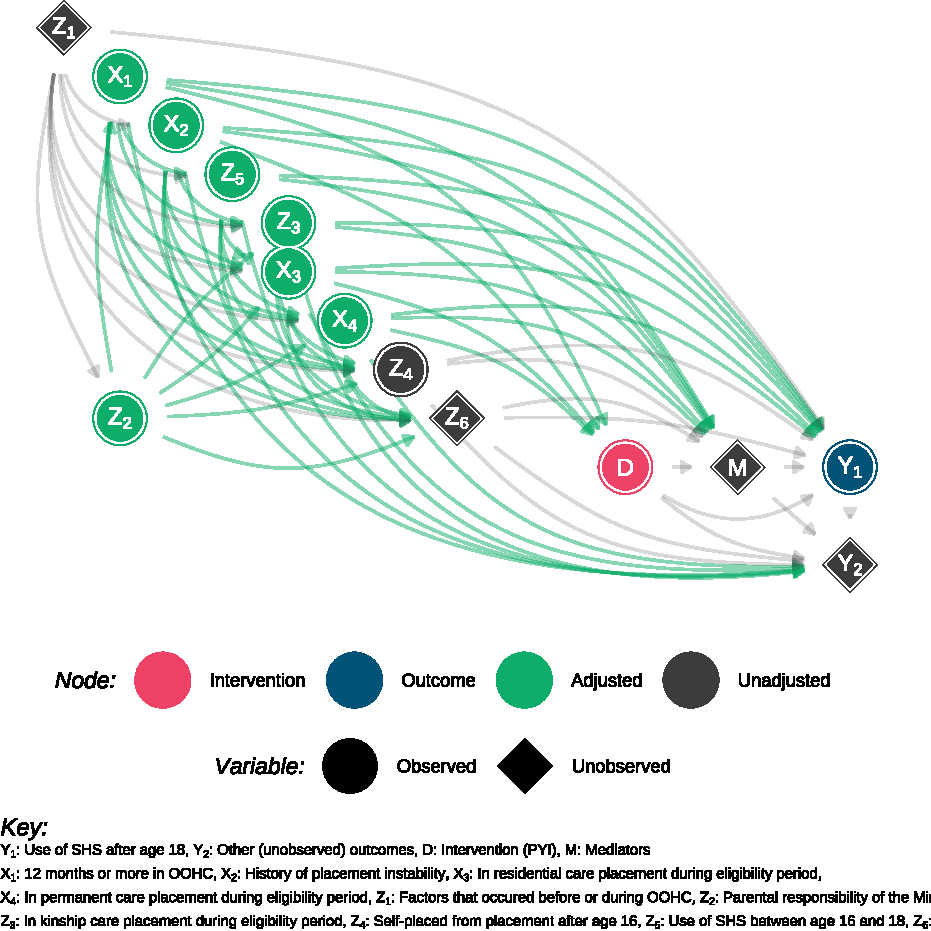
\includegraphics[keepaspectratio]{pyi_manuscript_files/figure-pdf/fig-pyi-dag-1.pdf}}

\end{figure*}

\subsection{Propensity Score Matching
Specification}\label{propensity-score-matching-specification}

We implemented propensity score matching using a series of iterative
specifications to achieve covariate balance. Propensity scores were
estimated using a generalised additive model (GAM) with a probit link
function using the \texttt{MatchIt} package
(\citeproc{ref-ho2011matchitnonparametricpreprocessing}{Ho, Imai, King,
\& Stuart, 2011}). The model included both our minimal adjustment set
\(X_i\) derived from our DAG and four additional pre-treatment
covariates \(Z_i\) that improved balance without introducing confounding
or collider bias (see Figure S1).

We applied two matching approaches: 1) 1:1 Nearest Neighbour, where each
treated unit was matched to a single comparison unit with the closest
propensity score, and 2) full matching, which optimally partitions the
full sample into matched sets containing one treated unit and a variable
number of weighted comparison units. In both specifications, matching
was done without replacement and comparison units outside the region of
common support were trimmed. No treated units were excluded.

\subsection{Treatment Effect
Estimation}\label{treatment-effect-estimation}

Treatment effects were estimated for binary, count, and continuous
outcome measures using logistic, Poisson, and linear regression models
respectively. Each model included the minimal adjustment set of
covariates derived from our DAG \(X_i\), as it has been shown to reduce
dependence on the specification of the matching model, while potentially
increasing precision and reducing bias from any residual imbalance
(\citeproc{ref-ho2007matchingnonparametricpreprocessing}{Ho, Imai, King,
\& Stuart, 2007}). We do not include the additional covariates \(Z_i\)
in our model since \(X_i\) is sufficient for identification.

Our general regression model specification took the form:

\begin{center}
$g(E[Y_i]) = \beta_0 + \beta_1 D_i + X_i'\beta$
\end{center}

where \(Y_i\) is the outcome for individual \(i\), \(D_i\) is the
treatment indicator, \(X_i\) is the vector of covariates representing
our minimal adjustment set, and \(g(.)\) is the appropriate link
function (identity for continuous outcomes, log for count outcomes, and
logit for binary outcomes).

The ATT was estimated using \emph{g}-computation
(\citeproc{ref-snowden2011implementationgcomputationsimulated}{Snowden,
Rose, \& Mortimer, 2011}) using the \texttt{marginaleffects} package
(\citeproc{ref-arel-bundock2024howinterpretstatistical}{Arel-Bundock,
Greifer, \& Heiss, 2024}). Standard errors (SE) and confidence intervals
(CI) were estimated using cluster-robust methods that account for
dependence between matched sets
(\citeproc{ref-abadie2022robustpostmatchinginference}{Abadie \& Spiess,
2022}). For non-linear models, where the delta method provides only
approximate standard errors, we used a cluster bootstrap with 4,999
replications (\citeproc{ref-austin2014usebootstrappingwhen}{Austin \&
Small, 2014}).

\subsubsection{Treatment Effect
Heterogeneity}\label{treatment-effect-heterogeneity}

To test for treatment effect heterogeneity, we plotted individual
treatment effect estimates against their propensity scores, following
Rosenbaum and Rubin
(\citeproc{ref-rosenbaum1983centralrolepropensity}{1983}). We examined
these plots to see if the fitted lines for the treatment and comparison
groups visibly differed across the range of the propensity score and
thus reveal potential effect moderators.

\subsubsection{Subgroup Analysis}\label{subgroup-analysis}

Conditional average treatment effects (CATTs) were estimated for two
pre-specified subgroups: Sex and Aboriginal and Torres Strait Islander
status. Subgroup analyses were also undertaken for variables where the
heterogeneity diagnostics suggested the potential for meaningful effect
modification. All CATTs were estimated with the full sample using
subgroup-treatment interaction terms. Given the small samples and rare
outcomes, we used parsimonious specifications without additional
covariates. For binary outcomes, we applied maximum penalised likelihood
with powers of the Jeffreys prior as penalty to reduce bias using the
\texttt{brglm2} package
(\citeproc{ref-kosmidis2021jeffreyspriorpenaltyfiniteness}{Kosmidis \&
Firth, 2021}).

\subsubsection{Sensitivity Analysis}\label{sensitivity-analysis}

We assessed sensitivity to unmeasured confounding using tipping point
analysis (\citeproc{ref-mcgowan2022tiprpackagesensitivity}{McGowan,
2022}) to determine the strength of confounding required to nullify our
findings.

\subsection{Implementation Analysis}\label{implementation-analysis}

\subsubsection{Data Collection}\label{data-collection}

We examined implementation through focus groups and interviews with key
stakeholders (October 2019-August 2020): PYI participants (8 focus
groups, n=36), PYI service and housing providers (8 focus groups and 6
interviews, n=42 participants), and funder representatives (5 focus
groups, n=15). Data collection protocols were informed by the
Consolidated Framework for Implementation Research (CFIR)
(\citeproc{ref-damschroder2009fosteringimplementationhealth}{Damschroder
et al., 2009}). Participant characteristics and data collection
protocols are provided in the supplementary material (sections
S3.2-S3.4).

\subsubsection{Qualitative analysis
framework}\label{qualitative-analysis-framework}

A modified version of the CFIR framework was used to examine
implementation barriers and facilitators at four critical junctures in
the client journey: intervention entry, pre-leaving care, transition
period, and independent living. Analysis followed a four-step process:
data familiarisation, application of both CFIR-derived and emergent
codes, categorisation of themes into barriers and facilitators, and
synthesis across stakeholder perspectives. We used data convergence to
triangulate findings across stakeholder groups to determine the
alignment of conclusions
(\citeproc{ref-palinkas2011mixedmethoddesigns}{Palinkas et al., 2011}).
A separate thematic analysis examined intervention acceptability through
participant perspectives on relationships with workers, support
effectiveness, service appropriateness, and social connections.

\section{Results}\label{results}

\subsection{Population
characteristics}\label{population-characteristics}

Characteristics of individuals who received PYI (n=295) are summarised
in Table 1. They were evenly distributed by sex (49.1\% male, 50.9\%
female). Despite forming 7.6\% of the NSW population aged 15-19 in 2021
(\citeproc{ref-abs2023populationestimatesage}{ABS, 2023},
\citeproc{ref-abs2024estimatedresidentpopulation}{2024}), almost a third
(32.9\%) of participants were Aboriginal and Torres Strait Islander
youth, which reflects their ongoing over representation in OOHC in
Australia. Since we relied on administrative data to identify
eligibility for the intervention over time, and we lack detail for when
an individual commenced the intervention, we looked at their
characteristics during the period they were eligible for the
intervention (aged between 16 years, 9 months to 17 years, 6 months)
rather than at a fixed baseline. Among eligibility criteria for the
intervention, which were not mutually exclusive, almost all had
experienced placement instability or had been in OOHC for twelve months
or more. The mean duration of time in OOHC at the start of their
eligibility period was \textasciitilde9 years. During the period at
which they were eligible, placements were distributed across residential
care (20.7\%), foster care (43.1\%), and kinship care (31.2\%). Notably,
30.9\% of participants had experienced at least one spell in SHS between
ages 16-18.

\begin{ThreePartTable}

\begin{table}

\caption{\label{tbl-one}Baseline characteristics of intervention group}

\centering{

\centering
\begin{talltblr}[         %% tabularray outer open
entry=none,label=none,
note{a}={Eligibility criteria for intervention},
note{b}={N (\%)},
note{c}={Mean (SD)},
]                     %% tabularray outer close
{                     %% tabularray inner open
colspec={Q[]Q[]},
cell{3}{1}={c=2}{},cell{6}{1}={c=2}{},cell{9}{1}={c=2}{},cell{14}{1}={c=2}{},cell{19}{1}={c=2}{},
column{2}={}{font=\fontsize{0.9em}{1.2em}\selectfont,},
row{1}={}{font=\fontsize{0.9em}{1.2em}\selectfont,},
cell{3}{1}={}{cmd=\textit, fg=c000000, font=\fontsize{0.9em}{1.2em}\selectfont,},
cell{6}{1}={}{cmd=\textit, fg=c000000, font=\fontsize{0.9em}{1.2em}\selectfont,},
cell{9}{1}={}{cmd=\textit, fg=c000000, font=\fontsize{0.9em}{1.2em}\selectfont,},
cell{14}{1}={}{cmd=\textit, fg=c000000, font=\fontsize{0.9em}{1.2em}\selectfont,},
cell{19}{1}={}{cmd=\textit, fg=c000000, font=\fontsize{0.9em}{1.2em}\selectfont,},
cell{2}{1}={}{preto={\hspace{1em}}, font=\fontsize{0.9em}{1.2em}\selectfont,},
cell{4}{1}={}{preto={\hspace{1em}}, font=\fontsize{0.9em}{1.2em}\selectfont,},
cell{5}{1}={}{preto={\hspace{1em}}, font=\fontsize{0.9em}{1.2em}\selectfont,},
cell{7}{1}={}{preto={\hspace{1em}}, font=\fontsize{0.9em}{1.2em}\selectfont,},
cell{8}{1}={}{preto={\hspace{1em}}, font=\fontsize{0.9em}{1.2em}\selectfont,},
cell{10}{1}={}{preto={\hspace{1em}}, font=\fontsize{0.9em}{1.2em}\selectfont,},
cell{11}{1}={}{preto={\hspace{1em}}, font=\fontsize{0.9em}{1.2em}\selectfont,},
cell{12}{1}={}{preto={\hspace{1em}}, font=\fontsize{0.9em}{1.2em}\selectfont,},
cell{13}{1}={}{preto={\hspace{1em}}, font=\fontsize{0.9em}{1.2em}\selectfont,},
cell{15}{1}={}{preto={\hspace{1em}}, font=\fontsize{0.9em}{1.2em}\selectfont,},
cell{16}{1}={}{preto={\hspace{1em}}, font=\fontsize{0.9em}{1.2em}\selectfont,},
cell{17}{1}={}{preto={\hspace{1em}}, font=\fontsize{0.9em}{1.2em}\selectfont,},
cell{18}{1}={}{preto={\hspace{1em}}, font=\fontsize{0.9em}{1.2em}\selectfont,},
cell{20}{1}={}{preto={\hspace{1em}}, font=\fontsize{0.9em}{1.2em}\selectfont,},
cell{21}{1}={}{preto={\hspace{1em}}, font=\fontsize{0.9em}{1.2em}\selectfont,},
cell{22}{1}={}{preto={\hspace{1em}}, font=\fontsize{0.9em}{1.2em}\selectfont,},
cell{23}{1}={}{preto={\hspace{1em}}, font=\fontsize{0.9em}{1.2em}\selectfont,},
cell{24}{1}={}{preto={\hspace{1em}}, font=\fontsize{0.9em}{1.2em}\selectfont,},
}                     %% tabularray inner close
\tinytableDefineColor{c000000}{HTML}{000000}
\toprule
Characteristic & Value \\ \midrule %% TinyTableHeader
Sample size (n)                                                  & 295           \\
Sex: & \\
Male                                                             & 145 (49.15)  \textsuperscript{b} \\
Female                                                           & 150 (50.85)  \textsuperscript{b} \\
Aboriginal and Torres Strait Islander status: & \\
Aboriginal or Torres Strait Islander                             & 97 (32.88)   \textsuperscript{b} \\
Non-Aboriginal or Torres Strait Islander                         & 198 (67.12)  \textsuperscript{b} \\
Current placement type during eligible period: & \\
Residential care placement                                      \textsuperscript{a} & 61 (20.68)   \textsuperscript{b} \\
Foster care placement                                            & 127 (43.05)  \textsuperscript{b} \\
Kinship care placement                                           & 92 (31.19)   \textsuperscript{b} \\
Permanent placement                                             \textsuperscript{a} & 218 (73.9)   \textsuperscript{b} \\
Out-of-home care experience: & \\
Parental responsibility of the Minister                          & 287 (97.29)  \textsuperscript{b} \\
Twelve months or more in out-of-home care                       \textsuperscript{a} & 292 (98.98)  \textsuperscript{b} \\
History of out-of-home care placement instability               \textsuperscript{a} & 292 (98.98)  \textsuperscript{b} \\
Months spent in care at point at which eligible for intervention & 107.36 (54.6)\textsuperscript{c} \\
Events after age 16: & \\
Placement breakdown                                              & 65 (22.03)   \textsuperscript{b} \\
Placement ended due to disruptive behaviour                      & 107 (36.27)  \textsuperscript{b} \\
Self-placed, missing or absent from placement                    & 54 (18.31)   \textsuperscript{b} \\
Independent living placement                                     & 59 (20)      \textsuperscript{b} \\
Spell in homelessness services                                   & 91 (30.85)   \textsuperscript{b} \\
\bottomrule
\end{talltblr}

}

\end{table}%

\end{ThreePartTable}

\subsection{Matching results}\label{matching-results}

We evaluated multiple matching algorithms (nearest neighbour, full,
optimal pair, and genetic matching) and propensity score estimation
methods (generalised linear models, gradient boosting, random forests,
and GAMs with various link functions). While nearest neighbour matching
with a probit-link GAM achieved good balance for most covariates, one
variable exceeded the conventional standardised mean difference (SMD)
threshold of 0.1. Applying full matching to the same model improved
balance across all covariates but reduced the effective sample size
(ESS). The final specification yielded an ESS of 196.8---representing
the equivalent number of equally weighted comparison units---compared to
295 in the nearest neighbour specification (see
Table~\ref{tbl-matching-results}). This highlights the bias-variance
trade-off: nearest neighbour matching offers greater precision through a
larger sample, whereas full matching minimises bias by improving
covariate balance, albeit at the cost of increased variance. Given our
primary goal was to reduce bias through optimal covariate balance, we
selected full matching as our preferred specification. Balance
diagnostics, including covariate balance (Figure S1) and common support
(Figure S2) for both specifications are available in the supplementary
material.

\begin{ThreePartTable}

\begin{table}

\caption{\label{tbl-matching-results}Results from two selected matching
specifications}

\centering{

\centering
\begin{tblr}[         %% tabularray outer open
]                     %% tabularray outer close
{                     %% tabularray inner open
width={1\linewidth},
colspec={X[0.261363636363636]X[0.102272727272727]X[0.102272727272727]X[0.0909090909090909]X[0.0909090909090909]X[0.0795454545454545]X[0.136363636363636]X[0.136363636363636]},
column{1,3,5,6,7,8}={}{font=\fontsize{0.9em}{1.2em}\selectfont,},
row{2,3,4}={}{font=\fontsize{0.9em}{1.2em}\selectfont,},
cell{1}{2}={c=2,}{font=\fontsize{0.9em}{1.2em}\selectfont, halign=c,},
cell{1}{4}={c=5,}{font=\fontsize{0.9em}{1.2em}\selectfont, halign=c,},
}                     %% tabularray inner close
\toprule
& Intervention &  & Comparison &  &  &  &  \\ \cmidrule[lr]{2-3}\cmidrule[lr]{4-8}
Specification & PYI sample & PYI matched & Sample & Matched & ESS & Unmatched & Discarded \\ \midrule %% TinyTableHeader
Nearest Neighbour & 295 & 295 & 422 & 295 & -     & 127 &  0 \\
Full matching     & 295 & 295 & 422 & 406 & 196.8 &   0 & 16 \\
\bottomrule
\end{tblr}

}

\end{table}%

\end{ThreePartTable}

\subsection{Effectiveness results}\label{effectiveness-results}

\subsubsection{Overall results}\label{overall-results}

Table~\ref{tbl-att-results} reports the ATT for each of the ten
outcomes, under both full and nearest-neighbour matching specifications.
As recommended by Westreich and Greenland
(\citeproc{ref-westreich2013table2fallacy}{2013}), we did not interpret
(or report) the individual regression coefficients, which lack
meaningful causal interpretation given our goal is to estimate the
treatment effect.

All outcomes represent negative events (e.g., entry into a SHS spell),
therefore a negative ATT estimate favours PYI. However, the observed
estimates typically centre near zero, with confidence intervals
comfortably spanning no effect, suggesting that on average, PYI does not
meaningfully shift the likelihood or magnitude of these outcomes
relative to the comparison group. Given that these events occur in only
approximately five percent of the sample, their rarity, along with the
relatively small sample size, may hinder detection of small or subtle
effects. Notably, the results are highly consistent across both matching
specifications, reinforcing the conclusion that there is no large or
systematic difference attributable to PYI.

To facilitate interpretation and synthesis, we have reported results in
multiple formats---for both full (Table S8) and nearest neighbour (Table
S9) specifications in the supplementary material. For binary outcomes,
we report risk differences (RD), relative risks (RR), and odds ratios
(OR). For count outcomes, we present both the raw mean difference and
its standardised form (Cohen's \emph{d}). For continuous outcomes, we
report mean differences in the natural units as well as Cohen's
\emph{d}. We have opted to provide this range of effect measures as a)
it allows readers to interpret results in their preferred metric, and b)
it may support including this study in future meta-analyses work. In
Figure~\ref{fig-pyi-smd}, we present a complete summary of our results,
including both matching specifications and all or our subgroup analyses,
with results visualised using Cohen's \emph{d} to place them on a common
scale.

\begin{twocolumntable}

\begin{table}

\caption{\label{tbl-att-results}ATT results for both matching
specifications}

\centering{

\centering
\begin{talltblr}[         %% tabularray outer open
entry=none,label=none,
note{a}={For binary outcomes, potential outcomes represent the estimated predicted probability of experiencing the outcome in each group (ranging from 0 to 1). The ATT represents the difference in these probabilities between groups (risk difference).},
note{b}={For continuous and count outcomes, potential outcomes represent the estimated mean value in each group. The ATT represents the mean difference between groups.},
]                     %% tabularray outer close
{                     %% tabularray inner open
width={1\linewidth},
colspec={X[0.571428571428571]X[0.0857142857142857]X[0.0857142857142857]X[0.0571428571428571]X[0.0571428571428571]X[0.142857142857143]},
cell{3}{1}={c=6}{},cell{14}{1}={c=6}{},
column{3,5,6}={}{font=\fontsize{0.8em}{1.1em}\selectfont,},
row{2}={}{font=\fontsize{0.8em}{1.1em}\selectfont,},
cell{1}{1}={}{font=\fontsize{0.8em}{1.1em}\selectfont,},
cell{3}{2}={}{font=\fontsize{0.8em}{1.1em}\selectfont,},
cell{3}{4}={}{font=\fontsize{0.8em}{1.1em}\selectfont,},
cell{4}{2}={}{font=\fontsize{0.8em}{1.1em}\selectfont,},
cell{4}{4}={}{font=\fontsize{0.8em}{1.1em}\selectfont,},
cell{5}{2}={}{font=\fontsize{0.8em}{1.1em}\selectfont,},
cell{5}{4}={}{font=\fontsize{0.8em}{1.1em}\selectfont,},
cell{6}{2}={}{font=\fontsize{0.8em}{1.1em}\selectfont,},
cell{6}{4}={}{font=\fontsize{0.8em}{1.1em}\selectfont,},
cell{7}{2}={}{font=\fontsize{0.8em}{1.1em}\selectfont,},
cell{7}{4}={}{font=\fontsize{0.8em}{1.1em}\selectfont,},
cell{8}{2}={}{font=\fontsize{0.8em}{1.1em}\selectfont,},
cell{8}{4}={}{font=\fontsize{0.8em}{1.1em}\selectfont,},
cell{9}{2}={}{font=\fontsize{0.8em}{1.1em}\selectfont,},
cell{9}{4}={}{font=\fontsize{0.8em}{1.1em}\selectfont,},
cell{10}{2}={}{font=\fontsize{0.8em}{1.1em}\selectfont,},
cell{10}{4}={}{font=\fontsize{0.8em}{1.1em}\selectfont,},
cell{11}{2}={}{font=\fontsize{0.8em}{1.1em}\selectfont,},
cell{11}{4}={}{font=\fontsize{0.8em}{1.1em}\selectfont,},
cell{12}{2}={}{font=\fontsize{0.8em}{1.1em}\selectfont,},
cell{12}{4}={}{font=\fontsize{0.8em}{1.1em}\selectfont,},
cell{13}{2}={}{font=\fontsize{0.8em}{1.1em}\selectfont,},
cell{13}{4}={}{font=\fontsize{0.8em}{1.1em}\selectfont,},
cell{14}{2}={}{font=\fontsize{0.8em}{1.1em}\selectfont,},
cell{14}{4}={}{font=\fontsize{0.8em}{1.1em}\selectfont,},
cell{15}{2}={}{font=\fontsize{0.8em}{1.1em}\selectfont,},
cell{15}{4}={}{font=\fontsize{0.8em}{1.1em}\selectfont,},
cell{16}{2}={}{font=\fontsize{0.8em}{1.1em}\selectfont,},
cell{16}{4}={}{font=\fontsize{0.8em}{1.1em}\selectfont,},
cell{17}{2}={}{font=\fontsize{0.8em}{1.1em}\selectfont,},
cell{17}{4}={}{font=\fontsize{0.8em}{1.1em}\selectfont,},
cell{18}{2}={}{font=\fontsize{0.8em}{1.1em}\selectfont,},
cell{18}{4}={}{font=\fontsize{0.8em}{1.1em}\selectfont,},
cell{19}{2}={}{font=\fontsize{0.8em}{1.1em}\selectfont,},
cell{19}{4}={}{font=\fontsize{0.8em}{1.1em}\selectfont,},
cell{20}{2}={}{font=\fontsize{0.8em}{1.1em}\selectfont,},
cell{20}{4}={}{font=\fontsize{0.8em}{1.1em}\selectfont,},
cell{21}{2}={}{font=\fontsize{0.8em}{1.1em}\selectfont,},
cell{21}{4}={}{font=\fontsize{0.8em}{1.1em}\selectfont,},
cell{22}{2}={}{font=\fontsize{0.8em}{1.1em}\selectfont,},
cell{22}{4}={}{font=\fontsize{0.8em}{1.1em}\selectfont,},
cell{23}{2}={}{font=\fontsize{0.8em}{1.1em}\selectfont,},
cell{23}{4}={}{font=\fontsize{0.8em}{1.1em}\selectfont,},
cell{24}{2}={}{font=\fontsize{0.8em}{1.1em}\selectfont,},
cell{24}{4}={}{font=\fontsize{0.8em}{1.1em}\selectfont,},
cell{3}{1}={}{font=\fontsize{0.8em}{1.1em}\selectfont, cmd=\textit, fg=c000000,},
cell{14}{1}={}{font=\fontsize{0.8em}{1.1em}\selectfont, cmd=\textit, fg=c000000,},
cell{4}{1}={}{preto={\hspace{1em}}, font=\fontsize{0.8em}{1.1em}\selectfont,},
cell{5}{1}={}{preto={\hspace{1em}}, font=\fontsize{0.8em}{1.1em}\selectfont,},
cell{6}{1}={}{preto={\hspace{1em}}, font=\fontsize{0.8em}{1.1em}\selectfont,},
cell{7}{1}={}{preto={\hspace{1em}}, font=\fontsize{0.8em}{1.1em}\selectfont,},
cell{8}{1}={}{preto={\hspace{1em}}, font=\fontsize{0.8em}{1.1em}\selectfont,},
cell{9}{1}={}{preto={\hspace{1em}}, font=\fontsize{0.8em}{1.1em}\selectfont,},
cell{10}{1}={}{preto={\hspace{1em}}, font=\fontsize{0.8em}{1.1em}\selectfont,},
cell{11}{1}={}{preto={\hspace{1em}}, font=\fontsize{0.8em}{1.1em}\selectfont,},
cell{12}{1}={}{preto={\hspace{1em}}, font=\fontsize{0.8em}{1.1em}\selectfont,},
cell{13}{1}={}{preto={\hspace{1em}}, font=\fontsize{0.8em}{1.1em}\selectfont,},
cell{15}{1}={}{preto={\hspace{1em}}, font=\fontsize{0.8em}{1.1em}\selectfont,},
cell{16}{1}={}{preto={\hspace{1em}}, font=\fontsize{0.8em}{1.1em}\selectfont,},
cell{17}{1}={}{preto={\hspace{1em}}, font=\fontsize{0.8em}{1.1em}\selectfont,},
cell{18}{1}={}{preto={\hspace{1em}}, font=\fontsize{0.8em}{1.1em}\selectfont,},
cell{19}{1}={}{preto={\hspace{1em}}, font=\fontsize{0.8em}{1.1em}\selectfont,},
cell{20}{1}={}{preto={\hspace{1em}}, font=\fontsize{0.8em}{1.1em}\selectfont,},
cell{21}{1}={}{preto={\hspace{1em}}, font=\fontsize{0.8em}{1.1em}\selectfont,},
cell{22}{1}={}{preto={\hspace{1em}}, font=\fontsize{0.8em}{1.1em}\selectfont,},
cell{23}{1}={}{preto={\hspace{1em}}, font=\fontsize{0.8em}{1.1em}\selectfont,},
cell{24}{1}={}{preto={\hspace{1em}}, font=\fontsize{0.8em}{1.1em}\selectfont,},
cell{1}{2}={c=2,}{font=\fontsize{0.8em}{1.1em}\selectfont, halign=c,},
cell{1}{4}={c=3,}{font=\fontsize{0.8em}{1.1em}\selectfont, halign=c,},
}                     %% tabularray inner close
\tinytableDefineColor{c000000}{HTML}{000000}
\toprule
& Estimated Potential Outcomes &  & Treatment Effect &  &  \\ \cmidrule[lr]{2-3}\cmidrule[lr]{4-6}
Outcome & Intervention group & Comparison group & ATT & SE & 95\% CI \\ \midrule %% TinyTableHeader
Full matching: &&&&& \\
In SHS spell on 18th birthday                                                                    \textsuperscript{a} & 0.047  & 0.067  & -0.02  & (0.022) & [-0.068, 0.019]  \\
In SHS spell on 19th birthday                                                                    \textsuperscript{a} & 0.064  & 0.051  & 0.013  & (0.022) & [-0.032, 0.055]  \\
New SHS spell between 18th \& 19th birthday                                                     \textsuperscript{a} & 0.142  & 0.142  & 0      & (0.03)  & [-0.06, 0.055]   \\
New or ongoing SHS spell between 18th \& 19th birthday                                          \textsuperscript{a} & 0.169  & 0.18   & -0.011 & (0.034) & [-0.076, 0.056]  \\
New unsheltered homelessness episode between 18th \& 19th birthday                              \textsuperscript{a} & 0.129  & 0.134  & -0.006 & (0.031) & [-0.074, 0.049]  \\
New or ongoing unsheltered homelessness episode between 18th and 19th birthday                   \textsuperscript{a} & 0.153  & 0.173  & -0.02  & (0.035) & [-0.09, 0.046]   \\
In new SHS spell that requires short term accommodation between 18th \& 19th birthday           \textsuperscript{a} & 0.142  & 0.142  & 0      & (0.03)  & [-0.06, 0.055]   \\
In new or ongoing SHS spell that requires short term accommodation between 18th \& 19th birthday\textsuperscript{a} & 0.169  & 0.18   & -0.011 & (0.034) & [-0.076, 0.056]  \\
Number of distinct SHS spells between 18th \& 19th birthday                                     \textsuperscript{b} & 0.227  & 0.351  & -0.124 & (0.079) & [-0.279, 0.031]  \\
Days in SHS spell between 18th \& 19th birthday                                                 \textsuperscript{b} & 15.427 & 18.725 & -3.298 & (4.931) & [-12.963, 6.368] \\
Nearest Neighbour matching: &&&&& \\
In SHS spell on 18th birthday                                                                    \textsuperscript{a} & 0.047  & 0.062  & -0.014 & (0.017) & [-0.049, 0.019]  \\
In SHS spell on 19th birthday                                                                    \textsuperscript{a} & 0.064  & 0.048  & 0.016  & (0.018) & [-0.02, 0.053]   \\
New SHS spell between 18th \& 19th birthday                                                     \textsuperscript{a} & 0.142  & 0.128  & 0.014  & (0.027) & [-0.038, 0.068]  \\
New or ongoing SHS spell between 18th \& 19th birthday                                          \textsuperscript{a} & 0.169  & 0.169  & 0      & (0.029) & [-0.057, 0.057]  \\
New unsheltered homelessness episode between 18th \& 19th birthday                              \textsuperscript{a} & 0.129  & 0.121  & 0.008  & (0.026) & [-0.043, 0.061]  \\
New or ongoing unsheltered homelessness episode between 18th and 19th birthday                   \textsuperscript{a} & 0.153  & 0.161  & -0.008 & (0.028) & [-0.063, 0.047]  \\
In new SHS spell that requires short term accommodation between 18th \& 19th birthday           \textsuperscript{a} & 0.142  & 0.128  & 0.014  & (0.027) & [-0.038, 0.068]  \\
In new or ongoing SHS spell that requires short term accommodation between 18th \& 19th birthday\textsuperscript{a} & 0.169  & 0.169  & 0      & (0.029) & [-0.057, 0.057]  \\
Number of distinct SHS spells between 18th \& 19th birthday                                     \textsuperscript{b} & 0.227  & 0.307  & -0.08  & (0.059) & [-0.196, 0.036]  \\
Days in SHS spell between 18th \& 19th birthday                                                 \textsuperscript{b} & 15.427 & 19.667 & -4.24  & (4.458) & [-12.979, 4.498] \\
\bottomrule
\end{talltblr}

}

\end{table}%

\end{twocolumntable}

\begin{figure*}[!htbp]

{\caption{{Treatment effect results for overall (ATT) and subgroup
analysis (CATT) presented as SMD for both matching
specifications}{\label{fig-pyi-smd}}}}

\pandocbounded{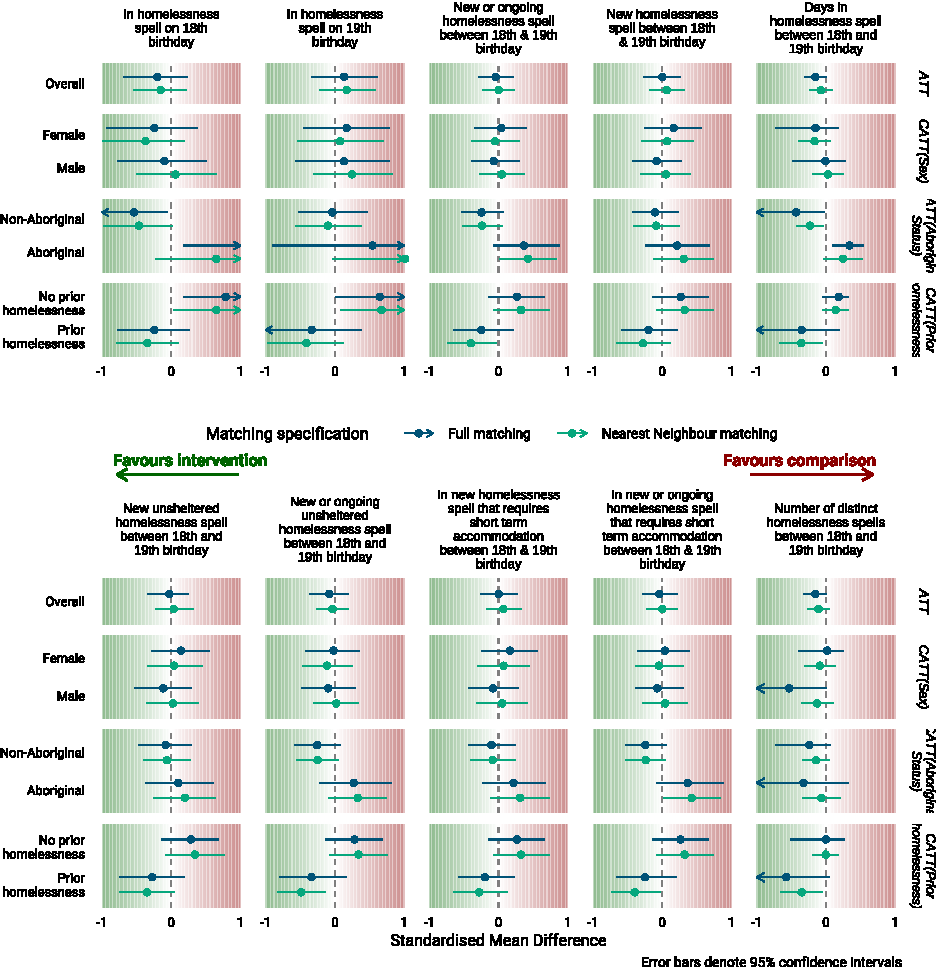
\includegraphics[keepaspectratio]{pyi_manuscript_files/figure-pdf/fig-pyi-smd-1.pdf}}

\end{figure*}

\paragraph{Treatment Effect
Heterogenity.}\label{treatment-effect-heterogenity}

We tested for treatment-effect heterogeneity in the ATT model and in six
additional conditional ATT analyses stratified by binary variables
included in the matching model (see Figures S3--S12). Across all ten
outcomes, heterogeneity emerged specifically for individuals who had
been homeless between ages 16 and 18 (hereafter `housing
vulnerability'). This pattern was observed in both matching
specifications, although it was more pronounced under full matching.
These findings suggest that housing vulnerability is a potential
moderator, warranting further examination through subgroup analysis.

\subsubsection{Subgroup Analyses}\label{subgroup-analyses}

Subgroup analysis was undertaken to estimate the conditional ATT (CATT)
on being male, Aboriginal or Torres Strait Islander or experiencing
housing vulnerability.

No difference was detected for the existence of moderation by sex (see
Tables S10 and S11) for results for both specifications.

We found that Aboriginal status moderates the treatment effect in four
of the ten examined outcomes in our full matching specification. For the
outcome in SHS on 18th birthday, Aboriginal participants experienced an
increased risk (CATT: 0.068, 95\% CI: {[}0.024, 0.126{]}), while
non-Aboriginal participants experienced a decrease (CATT: -0.057, 95\%
CI: {[}-0.126, -0.012{]}). The difference in risk differences (-0.125,
95\% CI: {[}-0.201, -0.049{]}, p = 0.001) provides some evidence of a
negative moderation effect. Similar patterns were observed for new or
ongoing SHS spell between 18th and 19th birthday (-0.164, 95\% CI:
{[}-0.308, -0.020{]}, p = 0.026), new or ongoing SHS spell requiring
short-term accommodation (-0.164, 95\% CI: {[}-0.308, -0.020{]}, p =
0.026), and days in SHS spell between 18th and 19th birthday (-29.651,
{[}-49.273, -10.029{]}, p = 0.003). In each of these cases, Aboriginal
participants experienced less favourable treatment effects compared to
their non-Aboriginal counterparts.

To put these results into context, for results reported as a risk
difference (RD), we can calculate the Number Needed to Treat (NNT) or
Number Needed to Harm (NNH) by taking the inverse of the point estimate
of the CATT (1/RD)
(\citeproc{ref-laupacis1988assessmentclinicallyuseful}{Laupacis,
Sackett, \& Roberts, 1988}). For Aboriginal participants, an NNH of
\textasciitilde15 (1/0.068 = 14.71) indicates that for every 15 youth
who received PYI, one additional youth will be in SHS on their 18th
birthday. Conversely, for non-Aboriginal participants, an NNT of
\textasciitilde18 (1/-0.057 = -17.54) means that 18 youth must receive
the intervention to prevent one additional youth from being in an SHS on
their 18th birthday. Results from the Nearest Neighbour specification
corroborated these results and identified similar moderation effects in
two additional outcomes (see Tables S12 and S13).

Moderation findings for housing vulnerability varied by matching
specification. Results from the nearest neighbour estimates suggest that
prior homelessness moderates the treatment effect in seven out of ten
outcomes (Table S14). Young people without prior homelessness
experienced a higher risk (CATT: 0.045, 95\% CI: {[}0.012, 0.088{]};
NNH: \textasciitilde22) of being in an SHS spell on their 19th birthday.
Whereas, those with prior homelessness were all at a lower risk of
experiencing a new or ongoing SHS spell between 18th and 19th birthday
(CATT: -0.173, 95\% CI: {[}-0.313, -0.018{]}; NNT: \textasciitilde6),
days in SHS spell between 18th and 19th birthday (CATT: -34.535, 95\%
CI: {[}-62.702, -6.368{]}), number of distinct SHS spells between 18th
and 19th birthday (CATT: -0.399, 95\% CI: {[}-0.754, -0.044{]}), a new
or ongoing SHS spell that requires short term accommodation (CATT:
-0.173, 95\% CI: {[}-0.313, -0.018{]}; NNT: \textasciitilde6), or new or
ongoing unsheltered homelessness spell (CATT: -0.203, 95\% CI:
{[}-0.340, -0.059{]}; NNT: \textasciitilde5).

The full matching estimates pointed in the same direction (see
Figure~\ref{fig-pyi-smd}), however they were subject to wider confidence
intervals that encompassed the null (Table S15). In other words, the
nearest neighbour results suggest potential heterogeneity in treatment
effects by housing vulnerability and the full matching results are
consistent with this possibility, however they are not detected at
conventional levels of statistical significance.

\subsubsection{Sensitivity Analyses}\label{sensitivity-analyses}

Since we did not detect any precise ATT estimates, we have included
results of our tipping point analysis in section S4.3 of the
supplementary material.

\subsection{Implementation results}\label{implementation-results}

\subsubsection{Intervention
acceptability}\label{intervention-acceptability}

Intervention acceptability---defined as the perception among
stakeholders that an intervention is agreeable, palatable, or
satisfactory
(\citeproc{ref-proctor2011outcomesimplementationresearch}{Proctor et
al., 2011})---was examined through focus groups with participants.
Thematic analysis revealed that participants' perceptions of
acceptability were largely shaped by four interconnected domains:
relationships with workers, effectiveness of support, appropriateness of
services, and peer relationships. Firstly, participants often
highlighted the importance of strong, trusting connections with
frontline staff. Many felt that workers' empathy, consistency, and
willingness to listen were central to the intervention's overall value,
particularly during critical junctures like entry into the intervention
and preparation for leaving care. As one participant shared ``They
listen more than they talk\ldots{} and they ask us what we want\ldots{}
we have a choice about what we want to do\ldots{}''. Secondly, views on
the intervention's effectiveness centered on whether the support
provided aligned with participants' self-identified needs. They often
contrasted the way in which PYI providers supported them with negative
experiences from OOHC. As one participant noted: ``My {[}OOHC{]} case
worker changed so many times, these guys {[}PYI{]} really make things
happen''. While some described the assistance as timely and
well-tailored---particularly around housing navigation and life
skills---others expressed a desire for broader or more intensive
resources in areas such as mental health and longer-term stability.
Thirdly, participants commented on the appropriateness of services,
noting that a flexible, person-centered approach helped them feel
respected and acknowledged. At the same time, some participants wanted
clearer communication about eligibility, referrals, and ongoing support
options, underscoring the need for transparent and consistent processes.
Lastly, participants' interactions with one another were seen as an
influential factor. Positive peer relationships often reinforced
feelings of shared experience and mutual support. As one participant
observed ``We have a group chat where we can chat and swap tips\ldots{}
it's really helpful''.

\subsubsection{Barriers and
Facilitators}\label{barriers-and-facilitators}

Implementation barriers and facilitators were thematically explored
around four time points, reflecting a clients experience of the
intervention: a) engaging with PYI; b) in PYI and before they left OOHC;
c) as they transitioned from OOHC; and d) living independently in the
community.

Several barriers were identified during engagement with PYI. Firstly, as
a pilot, PYI and its providers were unfamiliar to many OOHC caseworkers,
leading to inconsistent engagement and delays in connecting eligible
youth to services. As one PYI provider shared ``If they {[}case
worker{]} didn't think their client needed PYI, or would benefit from
it, they wouldn't prioritise engaging with us\ldots{} it was really
frustrating''. Secondly, while young people with significant
disabilities that prevented them from living independently were
ineligible for PYI, this information was not captured in administrative
data, requiring time-consuming manual screening by PYI providers.
Finally, the closed referral pathway and the initial evaluation design
(RCT) initially created some suspicion at multiple levels of the OOHC
system in sites where PYI was provided. However, the structured
eligibility criteria and use of administrative data to identify eligible
young people was also identified as facilitating the identification of
at-risk youth---particularly those who self-placed--- who might have
been overlooked through standard referral channels. As one PYI provider
noted: ``Without it some of these kids would have fallen through the
cracks\ldots{} they didn't have a caseworker, they needed us to go
hunting for them.''

While young people were still in OOHC, the major barrier faced by PYI
providers was that many clients lacked basic aftercare preparation like
leaving care plans, identification documents, and access to financial
services --- despite statutory requirements for this to occur. As one
representative from DCJ noted ``DCJ has made it really difficult to get
`sign off' to leaving care plans\ldots{} PYI has helped us show this''.
This required PYI staff to divert time and resources toward securing
these basic entitlements rather than focusing on goal-setting and
attainment. Providers felt that engaging with care leavers at an earlier
age provided them with more time to build relationships and advocate for
aftercare support.

As they transitioned from OOHC, several structural barriers impacted
service delivery. Limited employment opportunities and appropriate
housing stock in regional areas made it difficult to support care
leavers to find either employment or housing. PYI's emphasis on private
rental market placements created implementation challenges, as providers
felt that this option wasn't suitable for all participants. As one PYI
housing provider explained, ``It's tough because kids don't normally
move out of home at 18 and here we have these kids, that are coming
straight out of care and into a private rental without knowing what's
normal functioning in a house.'' While accommodation was available
through PYI, providers reported underutilisation of allocated housing
slots despite perceived scarcity, suggesting a misalignment between
intervention design and local implementation contexts. Implementation
facilitators emerged through providers' adaptive responses. Success in
housing placement was achieved through developing relationships with
real estate agents and property owners. Providers enhanced service
integration by connecting participants with complementary supports
through vocational educational institutions that structured the delivery
of practical skill-building activities, particularly around budgeting
and tenancy management.

After young people left care the reliance on private rental markets
continued to be a barrier, where limited affordable housing stock
constrained providers' placement options. While shared housing was
utilised to address this barrier, implementation success varied based on
whether participants had choice in these arrangements. Service delivery
was further complicated by property management issues, particularly
around visitor-related damages, which strained provider relationships
with real estate agents. The absence of clear operational definitions
for ``success'' created implementation uncertainty, affecting both
service boundaries and exit planning. Implementation facilitators
centred on sustained worker engagement and ongoing flexible support.
Providers identified that young people required approximately 12 months
post-care to develop adequate support networks. Finally, providers
observed that they required 12-18 months to codify and deliver services
they perceived to be effective, highlighting the substantial time
investment needed to achieve stable intervention delivery.

\section{Discussion}\label{discussion}

\subsection{Key results}\label{key-results}

On average, the PYI intervention did not meaningfully alter the
likelihood or magnitude of homelessness-related outcomes for care
leavers between their 18th and 19th birthdays. Across ten measures of
the homelessness, point estimates were near zero, and confidence
intervals comfortably encompassed no effect. The rarity of these events
likely limited power to detect smaller effects, yet the consistency of
findings under both full and nearest‐neighbour matching reinforces the
absence of any large or systematic impact. While this suggests that PYI
may not dramatically shift short-term housing trajectories, it does not
categorically exclude more nuanced or longer-run effects.

The effectiveness of PYI differs meaningfully across participant
subgroups with evidence of treatment-effect heterogeneity emerged in two
substantively important domains. First, we observed that PYI's impact
may differ for those with a history of homelessness between ages 16 and
18 (i.e., housing vulnerability). Under nearest-neighbour matching,
these individuals appeared to benefit more from PYI compared with their
peers without such histories, although the confidence intervals for the
full matching specification crossed the null, signaling that we cannot
we confident about this result. Second, Aboriginal participants
exhibited less favourable responses to PYI relative to non-Aboriginal
participants. This pattern was evident under both matching approaches
and persisted across multiple measures. Our confidence in this finding
is limited by the uncertainty in the estimates, but even with this
uncertainty, we believe this pattern warrants highlighting.

Implementation of PYI was characterised by significant system-level
barriers despite strong acceptability among stakeholders and
identifiable facilitators of success. Thematic analysis reveals that
acceptability of the intervention was driven chiefly by strong
worker-participant relationships, perceived effectiveness of support,
appropriate service alignment with participants' needs, and the
potential for peer relationships to bolster mutual support. However,
intervention implementation encountered substantial barriers across four
key phases of engagement: from initial referral through to the
transition from OOHC and into independent living. Poor aftercare
planning and limited housing options---particularly within private
rental markets---were recurrent challenges that providers sought to
mitigate. Facilitators included the use of eligibility criteria and
administrative data to identify at-risk youth, developing relationships
with key stakeholders (e.g., real estate agents), and providing ongoing
support in a flexible manner.

\subsection{Interpretation}\label{interpretation}

Consistent with other impact evaluations, it may be that interventions
like PYI are delivered at the wrong time, to the wrong population, or
are not delivered at an intensity sufficient to help care leavers with
the many complex challenges that they face. In the case of PYI, the fact
that 31\% of those who received the intervention already had at least
one spell in SHS before turning 18 suggests that the intervention may
have been delivered too late to change their trajectory---at least in
the first 12 months post-exit. Assisting care leavers in their
transition to independence is a challenging area of practice, we know
that most TSP for care leavers have null effects, and if they do have an
impact, they tend to be small (Taylor et al., 2024). By focusing the
intervention on those care leavers who were at the highest risk, e.g.,
those who had previously self-placed or used SHS, it is possible that
PYI may have been able to be provided at a higher intensity.

It is promising that care leavers find PYI highly acceptable, suggesting
that they welcome the provision of supportive interventions like PYI. In
focus groups, participants often contrasted the perceived effectiveness
of the support they received through PYI relative to leaving care
planning they received from their OOHC caseworkers. Furthermore,
anecdotes from participants suggest that those who had self-placed were
more likely to engage with PYI.

The insufficient and/or poor leaving care planning identified by PYI
providers raises concerns, as these deficiencies crowded out the
delivery of core components of the intervention. Notably, these
shortcomings in leaving care planning by OOHC providers are consistent
with reviews by NSW Office of the Children's Guardian
(\citeproc{ref-officeofthechildrensguardian2022reportleavingcare}{2022})
and Victorian Commission for Children and Young People
(\citeproc{ref-commissionforchildrenandyoungpeople2020keepcaringsystemic}{2020}).

\subsection{Limitations}\label{limitations}

Several limitations must be acknowledged. Firstly, the scope of our
outcome data was limited to SHS use, which may overlook other relevant
outcomes such as employment, income support, arrests, convictions,
incarceration, unplanned pregnancies, and emergency department
presentations. Furthermore, we were only able to observe outcomes
between the ages of 18 (when participants left OOHC) and 19, a
relatively short window during which the trajectories of those receiving
PYI may not have fully diverged from their counterfactual. Additionally,
the use of administrative data captures only individuals who engage with
SHS, thus failing to account for those experiencing hidden homelessness
(e.g., couch surfing), potentially underestimating the true incidence of
housing instability
(\citeproc{ref-metraux2017usingadministrativedata}{Metraux \& Tseng,
2017}). Finally, as with any study relying on selection-on-observables,
the potential for unmeasured confounding must be acknowledged. Whilst we
are confident in our ability to account for the intervention's selection
criteria, we lack sufficient information to identify individuals in the
comparison group who are not capable of living independently. Young
people with health conditions or disabilities that prevent them from
living independently would have been ineligible for PYI. These
individuals were likely supported by a different system that includes
accommodation and would thus, comparatively, have a lower likelihood of
homelessness. Our inability to identify and exclude these individuals
from our comparison pool potentially biases our estimates toward
services as usual.

\subsection{Implications for practice and
policy}\label{implications-for-practice-and-policy}

With nearly one-third of PYI participants accessing SHS before leaving
care, interventions such as PYI---that are specifically designed to
prevent homelessness among care leavers---must begin earlier and be more
precisely targeted. Since PYI's inception, NSW has introduced extended
care until age 21, a scalable initiative appealing as a broad policy
option (\citeproc{ref-mendes2025introductionextendedoutofhome}{Mendes et
al., 2025}). Some evidence suggests extended care can reduce
homelessness among care leavers, but the evidence in favour is not
conclusive, especially with respect to heterogenous treatment effects
(\citeproc{ref-taylor2024systematicreviewmetaanalysis}{Taylor et al.,
2024}). Meanwhile, interventions like PYI pose scaling challenges and
may not be suited for broad adoption as a first-line strategy.

Poor aftercare planning has been identified as a practice issue in NSW
(\citeproc{ref-officeofthechildrensguardian2022reportleavingcare}{Office
of the Children's Guardian, 2022};
\citeproc{ref-taylor2020evaluationpremiersyouth}{Taylor et al., 2020}).
Quality improvement methods such as audit and feedback, which can
pinpoint and rectify deficiencies in service delivery, may be a viable
option to improve practice
(\citeproc{ref-grimshaw2019reinvigoratingstagnantscience}{Grimshaw et
al., 2019}). Care leavers are not a monolithic group. While extended
care could help some achieve a more stable transition to independent
living, it likely will not benefit others, particularly those already
disengaged from their placements. The use of predictive modelling with
administrative data could help identify high-risk care leavers earlier,
enabling more targeted, preemptive responses
(\citeproc{ref-cuccaro-alamin2017riskassessmentdecision}{Cuccaro-Alamin,
Foust, Vaithianathan, \& Putnam-Hornstein, 2017}).

\subsection{Implications for research}\label{implications-for-research}

Selection-on-observables approaches, such as matching, are widely used
in program evaluations, but the strong assumptions they require---namely
that all relevant confounders have been observed---often receive
insufficient scrutiny. To address this, we employed a DAG to make our
assumptions explicit. Use of a DAG does not guarantee freedom from
unmeasured confounding. However, it clarifies the causal pathways that
we hypothesise are present and enables others to assess potential biases
in our analysis, and we recommend their use. Likewise, we also recommend
application of the potential outcomes framework as it supplies a
transparent and formal means of framing a causal question. Finally, the
use of \emph{g}-computation can then help avoid the pitfalls of
misinterpreting regression coefficients, commonly known as the Table 2
fallacy (\citeproc{ref-westreich2013table2fallacy}{Westreich \&
Greenland, 2013}). Huntington-Klein
(\citeproc{ref-huntington-klein2022effectintroductionresearch}{2022})
and Cunningham
(\citeproc{ref-cunningham2021causalinferencemixtape}{2021}) provide
detailed, accessible and practical resources for practitioners
interested in applying such methods.

Looking ahead, there remains a pressing need to improve our
understanding of how care leavers and CEYP fare across critical
domains---such as education, employment, mental health, and housing
stability---at different ages so that we can develop policies and/or
interventions that provide appropriate support at the right time. Linked
administrative data offers excellent opportunities to undertake this
important epidemiological work. While administrative data may lack the
granular detail of surveys (or other qualitative approaches), the
ability to use it to follow an entire cohort makes it uniquely suited
for tracking care leavers, who can be hard-to-reach.

\section{Conclusion}\label{conclusion}

PYI did not significantly reduce homelessness for most participants. The
intervention was markedly less effective for Aboriginal young people,
although it did potentially benefit those with prior experience of
homelessness. We cannot definitively determine whether PYI's limited
impact stems from issues with the intervention's design, if it was
delivered at the wrong time or not implemented well.

Evaluating interventions like PYI is essential for advancing our
understanding of `what works', even (and perhaps especially) when
results show limited or no effect. In the absence of experimental
studies, careful application of observational methods, such as those
employed in this paper, can play a crucial role in building the evidence
base. By illuminating both the strengths and weaknesses of current
approaches, such work helps practitioners to refine future services and
ensures that support for care leavers is guided by the best available
evidence.

\section{References}\label{references}

\phantomsection\label{refs}
\begin{CSLReferences}{1}{0}
\bibitem[\citeproctext]{ref-abadie2022robustpostmatchinginference}
Abadie, A., \& Spiess, J. (2022). Robust {Post-Matching Inference}.
\emph{Journal of the American Statistical Association}, \emph{117}(538),
983--995. \url{https://doi.org/10.1080/01621459.2020.1840383}

\bibitem[\citeproctext]{ref-abs2023populationestimatesage}
ABS. (2023). \emph{Population estimates by age and sex, by {SA2}, 2023}.
Canberra: Australian Bureau of Statistics.

\bibitem[\citeproctext]{ref-abs2024estimatedresidentpopulation}
ABS. (2024). \emph{Estimated resident population, {Aboriginal} and
{Torres Strait Islander Australians}, sex and age groups by states and
territories and {Australia}---2011 to 2021}. Canberra: Australian Bureau
of Statistics.

\bibitem[\citeproctext]{ref-aihw2021incomesupportreceipt}
AIHW. (2021). \emph{Income support receipt for young people
transitioning from out-of-home care}. Canberra: {Australian Institute of
Health and Welfare}.

\bibitem[\citeproctext]{ref-aihw2022incomesupportreceipt}
AIHW. (2022). \emph{Income support receipt for young people
transitioning from out-of-home care 2022}. Canberra: {Australian
Institute of Health and Welfare}.

\bibitem[\citeproctext]{ref-aihw2023specialisthomelessnessservice}
AIHW. (2023). \emph{Specialist homelessness service usage and receipt of
income support for people transitioning from out-of-home care}.
Canberra: {Australian Institute of Health and Welfare}.

\bibitem[\citeproctext]{ref-arel-bundock2024howinterpretstatistical}
Arel-Bundock, V., Greifer, N., \& Heiss, A. (2024). How to {Interpret
Statistical Models Using} marginaleffects for {R} and {Python}.
\emph{Journal of Statistical Software}, \emph{111}, 1--32.
\url{https://doi.org/10.18637/jss.v111.i09}

\bibitem[\citeproctext]{ref-austin2014usebootstrappingwhen}
Austin, P. C., \& Small, D. S. (2014). The use of bootstrapping when
using propensity-score matching without replacement: A simulation study.
\emph{Statistics in Medicine}, \emph{33}(24), 4306--4319.
\url{https://doi.org/10.1002/sim.6276}

\bibitem[\citeproctext]{ref-benchimol2015reportingstudiesconducted}
Benchimol, E. I., Smeeth, L., Guttmann, A., Harron, K., Moher, D.,
Petersen, I., \ldots{} Committee, R. W. (2015). The {REporting} of
studies {Conducted} using {Observational Routinely-collected} health
{Data} ({RECORD}) {Statement}. \emph{PLOS Medicine}, \emph{12}(10),
e1001885. \url{https://doi.org/10.1371/journal.pmed.1001885}

\bibitem[\citeproctext]{ref-cashmore2007longitudinalstudywards}
Cashmore, J., \& Paxman, M. (2007). \emph{Longitudinal study of wards
leaving care: Four to five years on}. Sydney: Social Policy Research
Centre, University of New South Wales.

\bibitem[\citeproctext]{ref-commissionforchildrenandyoungpeople2020keepcaringsystemic}
Commission for Children and Young People. (2020). \emph{Keep caring:
{Systemic} inquiry into services for young people transitioning from
out-of-home care}. Melbourne: {Commission for Children and Young
People}.

\bibitem[\citeproctext]{ref-courtney2006earlyoutcomesyoung}
Courtney, M. E., \& Dworsky, A. (2006). Early outcomes for young adults
transitioning from out-of-home care in the {USA}. \emph{Child and Family
Social Work}, \emph{11}(3), 209--219.
\url{https://doi.org/10.1111/j.1365-2206.2006.00433.x}

\bibitem[\citeproctext]{ref-courtney2017potentialeducationalbenefits}
Courtney, M. E., \& Hook, J. L. (2017). The potential educational
benefits of extending foster care to young adults: {Findings} from a
natural experiment. \emph{Children and Youth Services Review},
\emph{72}, 124--132.
\url{https://doi.org/10.1016/j.childyouth.2016.09.030}

\bibitem[\citeproctext]{ref-cuccaro-alamin2017riskassessmentdecision}
Cuccaro-Alamin, S., Foust, R., Vaithianathan, R., \& Putnam-Hornstein,
E. (2017). Risk assessment and decision making in child protective
services: {Predictive} risk modeling in context. \emph{Children and
Youth Services Review}, \emph{79}, 291--298.
\url{https://doi.org/10.1016/j.childyouth.2017.06.027}

\bibitem[\citeproctext]{ref-cunningham2021causalinferencemixtape}
Cunningham, S. (2021). \emph{Causal {Inference}: {The Mixtape}}. New
Haven, CT: Yale University Press.

\bibitem[\citeproctext]{ref-curran2012effectivenessimplementationhybriddesigns}
Curran, G. M., Bauer, M., Mittman, B., Pyne, J. M., \& Stetler, C.
(2012). Effectiveness-implementation {Hybrid Designs}: {Combining
Elements} of {Clinical Effectiveness} and {Implementation Research} to
{Enhance Public Health Impact}. \emph{Medical Care}, \emph{50}(3),
217--226. \url{https://doi.org/10.1097/MLR.0b013e3182408812}

\bibitem[\citeproctext]{ref-damschroder2009fosteringimplementationhealth}
Damschroder, L. J., Aron, D. C., Keith, R. E., Kirsh, S. R., Alexander,
J. A., \& Lowery, J. C. (2009). Fostering implementation of health
services research findings into practice: {A} consolidated framework for
advancing implementation science. \emph{Implementation Science},
\emph{4}(50). \url{https://doi.org/10.1186/1748-5908-4-50}

\bibitem[\citeproctext]{ref-dcj2025yourchoiceyour}
DCJ. (2025). Your {Choice}, {Your Future} -- new aftercare supports for
carers.
https://dcj.nsw.gov.au/dcj/children-and-families/out-of-home-care/children-in-out-of-home-care/planning-for-your-future-and-support-after-care/your-choice-your-future.html;
NSW Government.

\bibitem[\citeproctext]{ref-elm2007strengtheningreportingobservational}
Elm, E. von, Altman, D. G., Egger, M., Pocock, S. J., Gøtzsche, P. C.,
\& Vandenbroucke, J. P. (2007). The {Strengthening} the {Reporting} of
{Observational Studies} in {Epidemiology} ({STROBE}) statement:
Guidelines for reporting observational studies. \emph{The Lancet},
\emph{370}(9596), 1453--1457.
\url{https://doi.org/10.1016/S0140-6736(07)61602-X}

\bibitem[\citeproctext]{ref-fixsen2005implementationresearchsynthesis}
Fixsen, D. L., Naoom, S. F., Blase, K. A., Friedman, R. M., \& Wallace,
F. (2005). \emph{Implementation {Research}: {A Synthesis} of the
{Literature}} (The \{\{National Implementation Research Network\}\} No.
FMHJ Publication \#231). Tampa FL: University of South Florida, Louis de
la Parte Florida Mental Health Institute.

\bibitem[\citeproctext]{ref-grimshaw2019reinvigoratingstagnantscience}
Grimshaw, J. M., Ivers, N., Linklater, S., Foy, R., Francis, J. J.,
Gude, W. T., \& Hysong, S. J. (2019). Reinvigorating stagnant science:
Implementation laboratories and a meta-laboratory to efficiently advance
the science of audit and feedback. \emph{BMJ Quality \& Safety},
\emph{28}(5), 416--423. \url{https://doi.org/10.1136/bmjqs-2018-008355}

\bibitem[\citeproctext]{ref-gypen2017outcomeschildrenwho}
Gypen, L., Vanderfaeillie, J., De Maeyer, S., Belenger, L., \& Van
Holen, F. (2017). Outcomes of children who grew up in foster care:
{Systematic-review}. \emph{Children and Youth Services Review},
\emph{76}, 74--83.
\url{https://doi.org/10.1016/j.childyouth.2017.02.035}

\bibitem[\citeproctext]{ref-ho2007matchingnonparametricpreprocessing}
Ho, D. E., Imai, K., King, G., \& Stuart, E. A. (2007). Matching as
{Nonparametric Preprocessing} for {Reducing Model Dependence} in
{Parametric Causal Inference}. \emph{Political Analysis}, \emph{15}(3),
199--236. \url{https://doi.org/10.1093/pan/mpl013}

\bibitem[\citeproctext]{ref-ho2011matchitnonparametricpreprocessing}
Ho, D. E., Imai, K., King, G., \& Stuart, E. A. (2011). {MatchIt}:
{Nonparametric Preprocessing} for {Parametric Causal Inference}.
\emph{Journal of Statistical Software}, \emph{42}(8), 1--28.

\bibitem[\citeproctext]{ref-huntington-klein2022effectintroductionresearch}
Huntington-Klein, N. (2022). \emph{The {Effect}: {An Introduction} to
{Research Design} and {Causality}}. Chapman \& Hall.

\bibitem[\citeproctext]{ref-kosmidis2021jeffreyspriorpenaltyfiniteness}
Kosmidis, I., \& Firth, D. (2021). Jeffreys-prior penalty, finiteness
and shrinkage in binomial-response generalized linear models.
\emph{Biometrika}, \emph{108}(1), 71--82.
\url{https://doi.org/10.1093/biomet/asaa052}

\bibitem[\citeproctext]{ref-laupacis1988assessmentclinicallyuseful}
Laupacis, A., Sackett, D. L., \& Roberts, R. S. (1988). An {Assessment}
of {Clinically Useful Measures} of the {Consequences} of {Treatment}.
\emph{New England Journal of Medicine}, \emph{318}(26), 1728--1733.
\url{https://doi.org/10.1056/NEJM198806303182605}

\bibitem[\citeproctext]{ref-mcgowan2022tiprpackagesensitivity}
McGowan, L. D. (2022). Tipr: {An R} package for sensitivity analyses for
unmeasured confounders. \emph{Journal of Open Source Software},
\emph{7}(77), 4495. \url{https://doi.org/10.21105/joss.04495}

\bibitem[\citeproctext]{ref-mendes2025introductionextendedoutofhome}
Mendes, P., Roche, S., Kristo, I., O'Donnell, M., Moore, T., Malvaso,
C., \ldots{} McDowall, J. J. (2025). The {Introduction} of {Extended
Out-of-Home Care} ({OOHC}) {Until} 21 {Years} in {Australia}: {A
Mapping} of {Policy}, {Legislation} and {Programs} in {Each
Jurisdiction}. \emph{Australian Journal of Social Issues}, 1--12.
\url{https://doi.org/10.1002/ajs4.389}

\bibitem[\citeproctext]{ref-metraux2017usingadministrativedata}
Metraux, S., \& Tseng, Y.-P. (2017). Using {Administrative Data} for
{Research} on {Homelessness}: {Applying} a {US Framework} to
{Australia}. \emph{Australian Economic Review}, \emph{50}(2), 205--213.
\url{https://doi.org/10.1111/1467-8462.12216}

\bibitem[\citeproctext]{ref-miller2020extendedfostercare}
Miller, M., Bales, D., \& Hirsh, M. (2020). \emph{Extended {Foster Care}
in {Washington State}: {Final Report}} {[}Document \{\{Number\}\}
20-05-3201{]}. Olympia, WA: Washington State Institute for Public
Policy.

\bibitem[\citeproctext]{ref-homesnsw2025youthinitiative}
NSW, H. (2025). Youth {Initiative}.
https://www.nsw.gov.au/departments-and-agencies/homes-nsw/housing-reforms-and-initiatives/youth-initiatives-housing-and-homelessness/youth-initiative;
NSW Government.

\bibitem[\citeproctext]{ref-nunez2022resiliencefactorsyouth}
Nuñez, M., Beal, S. J., \& Jacquez, F. (2022). Resilience factors in
youth transitioning out of foster care: {A} systematic review.
\emph{Psychological Trauma: Theory, Research, Practice, and Policy},
\emph{14}(S1), S72--S81. \url{https://doi.org/10.1037/tra0001096}

\bibitem[\citeproctext]{ref-officeofthechildrensguardian2022reportleavingcare}
Office of the Children's Guardian. (2022). \emph{Report on leaving care
monitoring program 2020-21}. Sydney: Office of the Children's Guardian.

\bibitem[\citeproctext]{ref-palinkas2011mixedmethoddesigns}
Palinkas, L. A., Aarons, G. A., Horwitz, S., Chamberlain, P., Hurlburt,
M., \& Landsverk, J. (2011). Mixed {Method Designs} in {Implementation
Research}. \emph{Administration and Policy in Mental Health and Mental
Health Services Research}, \emph{38}(1), 44--53.
\url{https://doi.org/10.1007/s10488-010-0314-z}

\bibitem[\citeproctext]{ref-petaja2022prevalencehighriskbehavior}
Petäjä, U.-K., Terkamo-Moisio, A., Karki, S., \& Häggman-Laitila, A.
(2022). The {Prevalence} of {High-Risk Behavior Among Adolescents} in
{Aftercare Services} and {Transitioning} from {Out-of-home Care}: {A
Systematic Review}. \emph{Adolescent Research Review}.
\url{https://doi.org/10.1007/s40894-022-00198-1}

\bibitem[\citeproctext]{ref-picker2024quasiexperimentalevaluationstaying}
Picker, V., Hirneis, V., \& Sanders, M. (2024). A {Quasi-Experimental
Evaluation} of the {Staying Put Intervention} for {Reducing Homelessness
Among Care Leavers}. \emph{European Journal of Homelessness},
\emph{18}(1).

\bibitem[\citeproctext]{ref-proctor2011outcomesimplementationresearch}
Proctor, E., Silmere, H., Raghavan, R., Hovmand, P., Aarons, G., Bunger,
A., \ldots{} Hensley, M. (2011). Outcomes for {Implementation Research}:
{Conceptual Distinctions}, {Measurement Challenges}, and {Research
Agenda}. \emph{Administration and Policy in Mental Health and Mental
Health Services Research}, \emph{38}(2), 65--76.
\url{https://doi.org/10.1007/s10488-010-0319-7}

\bibitem[\citeproctext]{ref-rcoreteam2024languageenvironmentstatistical}
R Core Team. (2024). \emph{R: {A} language and environment for
statistical computing}. Vienna: R Foundation for Statistical Computing.

\bibitem[\citeproctext]{ref-rosenbaum1983centralrolepropensity}
Rosenbaum, P. R., \& Rubin, D. B. (1983). The {Central Role} of the
{Propensity Score} in {Observational Studies} for {Causal Effects}.
\emph{Biometrika}, \emph{70}(1), 41--55.
\url{https://doi.org/10.2307/2335942}

\bibitem[\citeproctext]{ref-rubin1974estimatingcausaleffects}
Rubin, D. B. (1974). Estimating causal effects of treatments in
randomized and nonrandomized studies. \emph{Journal of Educational
Psychology}, \emph{66}(5), 688--701.
\url{https://doi.org/10.1037/h0037350}

\bibitem[\citeproctext]{ref-sanders2021homelessnesschildrenssocial}
Sanders, M., Jones, L., \& Whelan, E. (2021). Homelessness and
{Children}'s {Social Care} in {England}. \emph{European Journal of
Homelessness}, \emph{15}(3), 129--141.

\bibitem[\citeproctext]{ref-sanders2023impactslifelonglinks}
Sanders, M., \& Picker, V. (2023). \emph{The {Impacts} of {Lifelong
Links} on {Housing Outcomes} for {Young People Leaving Care}: {An}
evaluation using matching}. London: Centre for Homelessness Impact.

\bibitem[\citeproctext]{ref-snowden2011implementationgcomputationsimulated}
Snowden, J. M., Rose, S., \& Mortimer, K. M. (2011). Implementation of
{G-Computation} on a {Simulated Data Set}: {Demonstration} of a {Causal
Inference Technique}. \emph{American Journal of Epidemiology},
\emph{173}(7), 731--738. \url{https://doi.org/10.1093/aje/kwq472}

\bibitem[\citeproctext]{ref-spindle-jackson2024extendedfostercare}
Spindle-Jackson, A., Byrne, T., \& Collins, M. E. (2024). Extended
foster care and homelessness: {Assessing} the impact of the fostering
connections to success and increasing adoptions act on rates of
homelessness among youth. \emph{Children and Youth Services Review},
107820. \url{https://doi.org/10.1016/j.childyouth.2024.107820}

\bibitem[\citeproctext]{ref-strahl2021multinationalcomparisoncareleaving}
Strahl, B., van Breda, A. D., Mann-Feder, V., \& Schröer, W. (2021). A
multinational comparison of care-leaving policy and legislation.
\emph{Journal of International and Comparative Social Policy}, 1--16.
\url{https://doi.org/10.1017/ics.2020.26}

\bibitem[\citeproctext]{ref-taylor2024systematicreviewmetaanalysis}
Taylor, D., Albers, B., Mann, G., Lewis, J., Taylor, R., Mendes, P.,
\ldots{} Shlonsky, A. (2024). Systematic {Review} and {Meta-Analysis} of
{Policies} and {Interventions} that {Improve Health}, {Psychosocial},
and {Economic Outcomes} for {Young People Leaving} the {Out-of-Home Care
System}. \emph{Trauma, Violence, \& Abuse}, \emph{25}(5), 3534--3554.
\url{https://doi.org/10.1177/15248380241253041}

\bibitem[\citeproctext]{ref-taylor2020evaluationpremiersyouth}
Taylor, D., Roberts, J., Rose, V., Gyani, A., Harrigan, S., \& Shlonsky,
A. (2020). \emph{Evaluation of the {Premier}'s {Youth Initiative}:
{Final Report}}. Sydney: {Centre for Evidence and Implementation}.

\bibitem[\citeproctext]{ref-taylor2025examiningimpactaccommodation}
Taylor, D., Roberts, J., Rose, V., Gyani, A., \& Shlonsky, A. (2025).
Examining the impact of an {Accommodation} and {Support Intervention} in
reducing homelessness amongst {Care Leavers} in {Australia}: {A} hybrid
type-1 {Implementation-Effectiveness Study} using {Propensity Score}
methods - supplementary material.

\bibitem[\citeproctext]{ref-taylor2025connectingdotsusing}
Taylor, D., Roberts, J., \& Shlonsky, A. (2025). \emph{Connecting the
{Dots}: {Using} a {Modified Delphi Method} to {Develop} a {Directed
Acyclic Graph} to~evaluate the effectiveness of an~{Accommodation} and
{Support Intervention} for {Care Leavers}}. Unpublished Manuscript, Data
Matters, Monash University, Melbourne.

\bibitem[\citeproctext]{ref-thoemmes2011systematicreviewpropensity}
Thoemmes, F. J., \& Kim, E. S. (2011). A {Systematic Review} of
{Propensity Score Methods} in the {Social Sciences}. \emph{Multivariate
Behavioral Research}, \emph{46}(1), 90--118.
\url{https://doi.org/10.1080/00273171.2011.540475}

\bibitem[\citeproctext]{ref-westreich2013table2fallacy}
Westreich, D., \& Greenland, S. (2013). The {Table}~2 {Fallacy}:
{Presenting} and {Interpreting Confounder} and {Modifier Coefficients}.
\emph{American Journal of Epidemiology}, \emph{177}(4), 292--298.
\url{https://doi.org/10.1093/aje/kws412}

\end{CSLReferences}






\end{document}
